%%%%%%%%%%%%%%%%%%%%%%%%%%%%%%%%%%%%%%%%%
% Sullivan Business Report
% LaTeX Template
% Version 1.0 (May 5, 2022)
%
% This template originates from:
% https://www.LaTeXTemplates.com
%
% Author:
% Vel (vel@latextemplates.com)
%
% License:
% CC BY-NC-SA 4.0 (https://creativecommons.org/licenses/by-nc-sa/4.0/)
%
%%%%%%%%%%%%%%%%%%%%%%%%%%%%%%%%%%%%%%%%%

%----------------------------------------------------------------------------------------
%	CLASS, PACKAGES AND OTHER DOCUMENT CONFIGURATIONS
%----------------------------------------------------------------------------------------

\documentclass[
	a4paper, % Paper size, use either a4paper or letterpaper
	12pt, % Default font size, the template is designed to look good at 12pt so it's best not to change this
	%unnumberedsections, % Uncomment for no section numbering
]{include/CSSullivanBusinessReport}

\addbibresource{include/sample.bib} % BibLaTeX bibliography file

%-----------------------------------------------------------------------
%	REPORT INFORMATION
%-----------------------------------------------------------------------
\reporttitle{} % The report title to appear on the title page and page headers, do not create manual new lines here as this will carry over to page headers

\reportsubtitle{A professional layout featuring a large margin\\ and examples of typical business report content} % Report subtitle, include new lines if needed

\reportauthors{Template created by:\\\smallskip Vel (vel@latextemplates.com)} % Report authors/group/department, include new lines if needed

\reportdate{\today} % Report date, include new lines for additional information if needed

\rightheadercontent{
\includegraphics[width=3cm]{./include/creodocs_logo.pdf}} % The content in the right header, you may want to add your own company logo or use your company/department name or leave this command empty for no right header content

\def\tightlist{}
%------------------------------------------------------------------------

\begin{document}

%------------------------------------------------------------------------
%	TITLE PAGE
%------------------------------------------------------------------------
\thispagestyle{empty} % Suppress headers and footers on this page

\begin{fullwidth} % Use the whole page width
	\vspace*{-0.075\textheight} % Pull logo into the top margin
	
	\hfill
\includegraphics[width=5cm]{./include/creodocs_logo.pdf} % Company logo

	\vspace{0.15\textheight} % Vertical whitespace

	\parbox{0.9\fulltextwidth}{\fontsize{50pt}{52pt}\selectfont\raggedright\textbf{\reporttitle}\par} % Report title, intentionally at less than full width for nice wrapping. Adjust the width of the \parbox and the font size as needed for your title to look good.
	
	\vspace{0.03\textheight} % Vertical whitespace
	
	{\LARGE\textit{\textbf{\reportsubtitle}}\par} % Subtitle
	
	\vfill % Vertical whitespace
	
	{\Large\reportauthors\par} % Report authors, group or department
	
	\vfill\vfill\vfill % Vertical whitespace
	
	{\large\reportdate\par} % Report date
\end{fullwidth}

\newpage

%----------------------------------------------------------------------------------------
%	DISCLAIMER/COPYRIGHT PAGE
%----------------------------------------------------------------------------------------
\thispagestyle{empty} % Suppress headers and footers on this page

\begin{twothirdswidth} % Content in this environment to be at two-thirds of the whole page width
	\footnotesize % Reduce font size
	
	\subsection*{Disclaimer}

	Lorem ipsum dolor sit amet, consectetur adipiscing elit. Praesent porttitor arcu luctus, imperdiet urna iaculis, mattis eros. Pellentesque iaculis odio vel nisl ullamcorper, nec faucibus ipsum molestie. Sed dictum nisl non aliquet porttitor. Etiam vulputate arcu dignissim, finibus sem et, viverra nisl. Aenean luctus congue massa, ut laoreet metus ornare in. Nunc fermentum nisi imperdiet lectus tincidunt vestibulum at ac elit.
	
	\subsection*{Copyright}
	
	\textcopyright~[Year] [Company] 
	
	Copyright notice text\ldots In hac habitasse platea dictumst. Curabitur mattis elit sit amet justo luctus vestibulum. In hac habitasse platea dictumst. Pellentesque lobortis justo enim, a condimentum massa tempor eu. Ut quis nulla a quam pretium eleifend nec eu nisl. Nam cursus porttitor eros, sed luctus ligula convallis quis.
	
	\subsection*{Contact}
	
	Address Line 1\\
	Address Line 2\\
	Address Line 3
	
	Business Number 123456
	
	Contact: name@company.com
	
	\vfill % Push the following down to the bottom of the page
	
	\subsubsection*{Changelog}
	
	\scriptsize % Reduce font size further
	
	\begin{tabular}{@{} L{0.05\linewidth} L{0.15\linewidth} L{0.6\linewidth} @{}} % Column widths specified here, change as needed for your content
		\toprule
		v1.0 & 20XX-02-05 & Lorem ipsum dolor sit amet, consectetur adipiscing elit. Praesent porttitor arcu luctus, imperdiet urna iaculis, mattis eros.\\
		v1.1 & 20XX-02-27 & Pellentesque iaculis odio vel nisl ullamcorper, nec faucibus ipsum molestie.\\
		v1.2 & 20XX-03-15 & Sed dictum nisl non aliquet porttitor.\\
		\bottomrule
	\end{tabular}
\end{twothirdswidth}

\newpage

%----------------------------------------------------------------------------------------
%	TABLE OF CONTENTS
%----------------------------------------------------------------------------------------
\begin{twothirdswidth} % Content in this environment to be at two-thirds of the whole page width
	\tableofcontents % Output the table of contents, automatically generated from the section commands used in the document
\end{twothirdswidth}

\newpage

%----------------------------------------------------------------------------------------
%	SECTIONS
%----------------------------------------------------------------------------------------

\section{Entregables Fase I de la Visión AE de
SG}\label{sec:entregables-fase-i-de-la-visiuxf3n-ae-de-sg}

\begin{itemize}
\tightlist
\item
  \hyperref[documento-de-visiuxf3n]{Documento de Visión}
\end{itemize}

\newpage

\section{Documento de Visión}\label{sec:documento-de-visiuxf3n}

\subsection{Visión del Dominio de Sistemas de
Información}\label{sec:visiuxf3n-del-dominio-de-sistemas-de-informaciuxf3n}

\begin{quote}
\end{quote}

La Fase Tres (3) de la arquitectura empresarial (AE) de SG se divide en
dos partes principales: Arquitectura de Datos y Arquitectura de
Aplicaciones.

\paragraph{Objetivo de la Arquitectura de
Aplicaciones:}\label{sec:objetivo-de-la-arquitectura-de-aplicaciones}

El objetivo principal de la Arquitectura de Aplicaciones es desarrollar
las arquitecturas de sistemas de información objetivo (tanto de datos
como de aplicaciones) que soporten la arquitectura de negocio
(desarrollada en la Fase B) y que implementen la visión de arquitectura
inicial (establecida en la Fase A).

En términos más específicos, la arquitectura de aplicaciones busca:

\begin{itemize}
\tightlist
\item
  Definir la arquitectura de las aplicaciones (software) necesarias para
  soportar los procesos de negocio.
\item
  Identificar las funciones de negocio que deben ser soportadas por las
  aplicaciones.
\item
  Establecer la interacción y el flujo de información entre las
  diferentes aplicaciones.
\item
  Considerar aspectos como la escalabilidad, el rendimiento, la
  mantenibilidad y la seguridad de las aplicaciones.
\item
  Listar los capacidades de negocio (servicios de aplicación)
  relacionadas con las arquitecturas de aplicaciones de SG.
\end{itemize}

\paragraph{Relación con las Fases del
Proyecto}\label{sec:relaciuxf3n-con-las-fases-del-proyecto}

La Arquitectura de Aplicaciones no opera de forma aislada; está
intrínsecamente conectada con las fases anteriores y posteriores de la
arquitectura empresarial de Secretaria General Alcaldía Mayor de Bogotá:

\begin{itemize}
\tightlist
\item
  Relación con la Fase A (Visión de la Arquitectura): La Fase C toma
  como entrada principal la Visión de la Arquitectura, que establece el
  alcance, los objetivos de alto nivel, los principios de la
  arquitectura y la visión del negocio. La Arquitectura de Sistemas de
  Información debe alinearse y contribuir a la consecución de esta
  visión.
\item
  Relación con la Fase B (Arquitectura de Negocio): La Arquitectura de
  Negocio (procesos de negocio, funciones, organización, etc.) es el
  motor principal para la Fase C. La Arquitectura de Sistemas de
  Información se construye para soportar y habilitar los requisitos
  definidos en la Arquitectura de Negocio. Por ejemplo, los procesos de
  negocio definidos en la Fase B informarán las necesidades de datos y
  las funcionalidades de las aplicaciones en la Fase C.
\item
  Relación con la Fase D (Arquitectura Tecnológica): La Fase C
  proporciona los requisitos para la Fase D. La Arquitectura de Sistemas
  de Información (datos y aplicaciones) determina la tecnología
  subyacente (hardware, software de infraestructura, middleware, redes)
  que se necesitará para soportar las aplicaciones y gestionar los
  datos. La Fase D, por lo tanto, desarrollará la Arquitectura
  Tecnológica basándose en las necesidades identificadas en la Fase C.
\item
  Relación con la Fase E (Oportunidades y Soluciones) y Fase F
  (Planificación de la Migración): Las arquitecturas de datos y
  aplicaciones desarrolladas en la Fase C son insumos críticos para
  identificar oportunidades de implementación (Fase E) y para
  desarrollar el plan de migración (Fase F) de las arquitecturas
  actuales a las arquitecturas objetivo.
\item
  Relación con la Gestión de Requisitos (Requirements Management): La
  Gestión de Requisitos es una capacidad continua que atraviesa todas
  las fases del ADM. Los requisitos de los sistemas de información,
  capturados y gestionados, son fundamentales para guiar el desarrollo
  de las arquitecturas en la Fase C y para asegurar que la arquitectura
  final cumpla con las necesidades del negocio.
\end{itemize}

\paragraph{Requisitos Necesarios para su Realización (Entradas
Clave):}\label{sec:requisitos-necesarios-para-su-realizaciuxf3n-entradas-clave}

Para llevar a cabo la Fase C de manera efectiva, una empresa debe contar
con ciertos requisitos y entradas esenciales, que provienen
principalmente de las fases previas del proceso de AE:

\begin{itemize}
\tightlist
\item
  Requisitos de Negocio: Una comprensión clara y detallada de los
  requisitos de negocio, procesos de negocio, funciones y estructuras
  organizacionales definidos en la Fase B. Esto incluye, por ejemplo, el
  Catálogo de Requisitos (como se menciona en el documento ``TOGAF
  Catalogs Matrices and Diagrams.pdf'', página 60), que ``captura las
  cosas que la empresa necesita hacer para cumplir sus objetivos''.
\item
  Visión de la Arquitectura: La ``Visión de la Arquitectura''
  (Architectural Vision) y los ``Principios de la Arquitectura''
  establecidos en la Fase A, que guiarán las decisiones de diseño en la
  Fase C.
\item
  Arquitectura de Negocio de Línea Base y Objetivo: Los modelos de
  Arquitectura de Negocio actual y deseada (definidos en la Fase B), que
  servirán como punto de partida y destino para la Arquitectura de
  Sistemas de Información.
\item
  Metamodelo de Contenidos de la Arquitectura: Una comprensión y
  aplicación del metamodelo de contenidos de TOGAF (referenciado en
  ``TOGAF 9.2 - Content Metamodel.pdf''), que proporciona un marco
  estructurado para describir los artefactos de la arquitectura.
\item
  Principios de Arquitectura de Sistemas de Información: Principios
  específicos que guiarán el diseño de los datos y las aplicaciones,
  asegurando la coherencia y la alineación con los objetivos
  empresariales.
\item
  Capacidad de Arquitectura Empresarial: La infraestructura y los
  recursos necesarios para realizar actividades de arquitectura,
  incluyendo herramientas de modelado (como ArchiMate, Draw.io,
  compatible con TOGAF) y personal con las habilidades adecuadas.
\item
  Planes de Iteración y Nivel de Detalle: El alcance y el nivel de
  detalle requerido para la arquitectura de sistemas de información, que
  a menudo se define en la Fase de Visión y se refina a medida que
  avanza el proceso de AE. Esto puede incluir un enfoque iterativo para
  el desarrollo de la arquitectura, según lo discutido en ``ADM
  Guidelines \& Techniques.pdf'' (Capítulo 19: Applying Iteration to the
  ADM).
\end{itemize}

La arquitectura de aplicaciones es un pilar fundamental en la
transformación empresarial, traduciendo las necesidades de negocio en
soluciones tangibles de datos y aplicaciones, y preparando el terreno
para la selección de la tecnología subyacente.

\begin{figure}
\centering
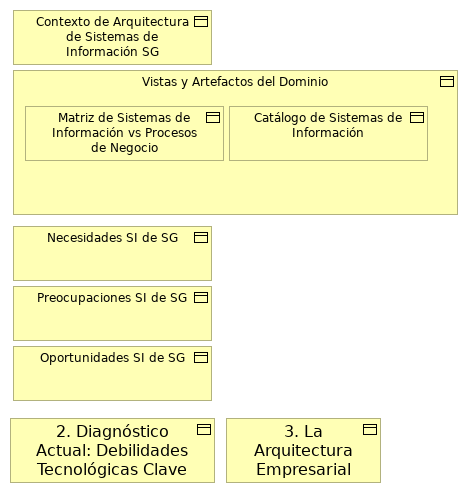
\includegraphics{images/06.3n.VisionSI.png}
\caption{06.3n. Vision SI. \emph{Fuente: Proyecto arquitectura
empresarial. Arquitectura de Aplicaciones Secretaria General Alcaldía
Mayor de Bogotá (2025)}}\label{fig:id-f46748634baa4f87afc7a9ab40892964}
\end{figure}

\subsubsection{Contexto de Arquitectura de Sistemas de Información
SG}\label{sec:contexto-de-arquitectura-de-sistemas-de-informaciuxf3n-sg}

Desde el dominio de aplicaciones y sistemas de información de la
Secretaría General, llamada en adelante ``la arquitectura de sistemas de
Información de SG'', buscamos adelantar las especificaciones de las
arquitecturas objetivo de los sistemas de información de Secretaria
General Alcaldía Mayor de Bogotá que soporten la arquitectura de negocio
y datos, en línea y dentro del alcance de la visión establecida en el
primer entregable de este ejercicio de arquitectura empresarial de SG
(AESG).

En particular, la arquitectura de sistemas de información de SG se
plantea, dentro del alcance de la visión del ejercicio:

\begin{itemize}
\tightlist
\item
  Definir la arquitectura de las aplicaciones (SI) necesarias para
  soportar los procesos de negocio de SG.
\item
  Identificar las funciones de negocio que deben ser soportadas por las
  aplicaciones de SG.
\item
  Establecer la interacción y el flujo de información entre las
  diferentes aplicaciones de SG.
\item
  Considerar aspectos sistémicos como la escalabilidad, el rendimiento,
  la mantenibilidad y la seguridad de las aplicaciones de SG.
\item
  Listar los capacidades de negocio (servicios de aplicación)
  relacionadas con las arquitecturas de aplicaciones de SG.
\end{itemize}

De esta manera, la arquitectura de sistemas de SG contribuye a la
consecución de la visión de este ejercicio de arquitectura empresarial
SG (AESG); y en lo específico, contribuye a los fines de la arquitectura
de negocio y tecnológica de SG, a delinear oportunidades y soluciones, y
a soportar la planeación de la migración. Todo lo anterior dentro del
alcance consignado en este ejercicio.

\paragraph{Alcance}\label{sec:alcance}

El presente ejercicio de la arquitectura dominio de aplicaciones toma
como alcance horizontal las áreas o unidades siguientes de la SG
(\emph{fuente: sesiones de levantamiento, entrevistas, y cuestionarios
compartidos en el mes de julio del 2025, junto con la recopilación
estructurada de las fuentes de información y organigramas}):

Unidades de negocio del alcance del dominio:

\begin{itemize}
\tightlist
\item
  Secretaría Privada

  \begin{itemize}
  \tightlist
  \item
    Oficina Consejería Distrital de Comunicación. César Augusto Castro
    Rodríguez
  \item
    Oficina Consejería Distrital de Tecnologías de la Información y las
    Comunicaciones -TIC. Diana Celis Mora
  \end{itemize}
\item
  Despacho del Secretario General. Miguel Andrés Silva Moyano

  \begin{itemize}
  \tightlist
  \item
    Oficina de Tecnologías de la Información y las Comunicaciones.
    Arleth Patricia Saurith Contreras
  \item
    Subsecretaría Distrital de Fortalecimiento Institucional. Alejandra
    Rodas Gaiter

    \begin{itemize}
    \tightlist
    \item
      Dirección Distrital de Desarrollo Institucional. Sebastian Estrada
      Jaramillo

      \begin{itemize}
      \tightlist
      \item
        Subdirección Técnica de Desarrollo Institucional. Diego Canesco
        Arenas
      \end{itemize}
    \end{itemize}
  \item
    Subsecretaría de Servicio a la Ciudadanía . Adriana Vargas Tamayo

    \begin{itemize}
    \tightlist
    \item
      Dirección del Sistema Distrital de Servicio a la Ciudadanía.
      Enrique Cusba García
    \end{itemize}
  \item
    Subsecretaría Corporativa. Henry Villamarín Serrano
  \item
    Subsecreataría de Servicios Ciudadanos (\ldots)
  \item
    Subsecreataría de Inversión y FF (\ldots)
  \item
    Subsecreataría de Operaciones
  \item
    Subsecreataría de Relaciones Internacionales (\ldots)
  \end{itemize}
\end{itemize}

En cuanto al alcance vertical, las aplicaciones de software que están
consignadas en este ejercicio son las siguientes (\emph{fuente: sesiones
de levantamiento, entrevistas, y cuestionarios compartidos en el mes de
julio del 2025, junto con la recopilación estructurada de las fuentes de
información}):

\begin{itemize}
\tightlist
\item
  Administrativo y Financiero: Soporta la gestión financiera, gestión de
  servicios administrativos y tecnológicos, y gestión de recursos
  físicos
\item
  Bogotá Te Escucha: Es fundamental para el proceso de Gobierno abierto
  y relacionamiento con la ciudadanía5. También se menciona como el
  Sistema Distrital para la Gestión de Peticiones Ciudadanas, a través
  del cual se evalúa la calidad de las respuestas emitidas a la
  ciudadanía
\item
  Bogotá Aprende TIC: Apoya los procesos de Gobierno abierto y
  relacionamiento con la ciudadanía, y Fortalecimiento de la Gestión
  Pública
\item
  DARUMA: Se utiliza en el proceso de Fortalecimiento de la Gestión
  Pública5. También es el aplicativo donde se encuentran definidas las
  fichas técnicas de productos y servicios de la Secretaría General8 y
  se gestionan los riesgos estratégicos
\item
  SIGA: Interviene en la gestión de contratación, gestión financiera,
  gestión de servicios administrativos y tecnológicos, y gestión de
  recursos físicos
\item
  SAT Web: Relacionado con la gestión de servicios administrativos y
  tecnológicos
\item
  GLOBO: Utilizado en el proceso de Fortalecimiento de la Gestión
  Pública
\item
  Datos para la Transparencia (SATI): Soporta el proceso de Gobierno
  abierto y relacionamiento con la ciudadanía
\item
  SUDIVC: Se aplica en los procesos de Gobierno abierto y
  relacionamiento con la ciudadanía, Paz, víctimas y reconciliación, y
  Fortalecimiento de la Gestión Pública
\item
  HUMANAPP: Apoya la gestión del talento humano
\item
  SIAB (El COFRE): Utilizado en los procesos de Gobierno abierto y
  relacionamiento con la ciudadanía, y Fortalecimiento de la Gestión
  Pública
\item
  KOHA: Relacionado con la Gestión del conocimiento
\item
  SIVIC: Interviene en los procesos de Paz, víctimas y reconciliación, y
  Fortalecimiento de la Gestión Pública
\item
  Data Warehouse AVANTI: Apoya la Gestión del conocimiento
\item
  Gestión Académica: Relacionado con la Gestión del conocimiento
\item
  EMLAZE: Utilizado en los procesos de Gobierno abierto y
  relacionamiento con la ciudadanía, y Fortalecimiento de la Gestión
  Pública
\item
  GLPI: Soporta la gestión de servicios administrativos y tecnológicos
\item
  GitLab: Se relaciona con la Gestión de alianzas e internacionalización
  de Bogotá
\end{itemize}

\subsubsection{Vistas y Artefactos del
Dominio}\label{sec:vistas-y-artefactos-del-dominio}

A continuación, presentamos las vistas y artefactos del dominio de
sistemas de información consignados en el alcance del proyecto.

\subsubsection{Matriz de Sistemas de Información vs Procesos de
Negocio}\label{sec:matriz-de-sistemas-de-informaciuxf3n-vs-procesos-de-negocio}

Las matrices del dominio de aplicaciones de software y sistemas de
información (SI) de SG son herramientas para el relacionamiento con
otros dominios del ejercicio de arquitectura empresarial de SG. Con esto
conseguimos soportar la toma decisiones de lo que debe ser compartido de
los SI dentro de la Secretaría, y entre sus aplicaciones de software.
Las matrices de este ejercicio sirven además para comunicar el grado de
relacionamiento de los elementos.

En resumen,

\begin{itemize}
\tightlist
\item
  Las matrices son cruciales para especificar cómo debe relacionarse la
  información entre los sistemas y otros dominios
\item
  proporcionan información crítica para los proyectos que involucren a
  los sistemas de SG.
\item
  Contribuye a la determinación de brechas (gaps) en las necesidades de
  compartir información (o funciones de los sistemas) ente los elementos
  de la matriz.
\item
  La matriz ayuda a definir el nivel de detalle de lo que se comparte.
\item
  Se deben establecer medidas similares para la interoperabilidad de
  servicios/negocios y la infraestructura (tecnología física).
\item
  Sintetizan la información de las arquitecturas, y son simples para
  compartir documentos.
\end{itemize}

Las matrices de este dominio (procesos e interoperabilidad) actúan como
una hoja de ruta para la conectividad y el intercambio de información;
inician desde una perspectiva de negocio de alto nivel y van hasta una
especificación técnica detallada del la interacción con los sistemas.
Sirven como herramienta de comunicación para los demás dominios de la
arquitectura empresarial de SG, y contribuyen a que las interacciones
relevantes entre servicios, canales, y procesos estén definidas y sean
compatibles.

\subsubsection{Catálogo de Sistemas de
Información}\label{sec:catuxe1logo-de-sistemas-de-informaciuxf3n}

En el contexto de TOGAF, El Catálogo de sistemas de información es un
inventario detallado y documentado que actúa como ficha técnica de los
sistemas de información o aplicaciones de software de SG.

Es un producto entregable clave de la fase de Arquitectura de
Aplicaciones dentro de la Fase 3 de este ejercicio de arquitectura
empresarial (AE). Forma parte del Marco de Referencia del Contenido
Arquitectónico de TOGAF y del Marco de Arquitectura de Referencia del
MinTIC (MAE 3.0, Colombia).

La construcción del catálogo de aplicaciones implican a las sesiones de
levantamiento, entrevistas, y cuestionarios compartidos en el mes de
julio, junto con la recopilación estructurada de las fuentes de
información sobre cada sistema.

\paragraph{Contenido Mínimo del
Catálogo}\label{sec:contenido-muxednimo-del-catuxe1logo}

\begin{itemize}
\tightlist
\item
  ID de Aplicación. Código de identificación de la aplicación de
  software.
\item
  Nombre de la Aplicación. Nombre de identificación de la aplicación de
  software.
\item
  Descripción. Funcionamiento básico de la aplicación de software.
\item
  Estado: {[}En producción, en desmantelamiento, en implementación,
  Inactiva{]}
\item
  Categoría: {[}Sistema de apoyo al negocio (misional), herramienta de
  gestión, Ofimática, Seguridad{]}
\item
  Proceso(s) de Negocio Clave(s)
\item
  Capacidad: Capacidades de nivel 2 relacionadas con la aplicación de
  software.
\item
  Tipo de aplicación: Web, Móvil, Cliente Servidor
\item
  Método de despliegue: on-premises, cloud SAAS, cloud PAAS, cloud IAAS
\item
  Tecnología. Aspectos técnicos de la aplicación de software.
\item
  Versión actual de la tecnología
\item
  Responsable técnico en la entidad
\item
  Responsable funcional en la entidad
\item
  Fabricante
\item
  Proveedor de soporte externo
\item
  Fecha de vigencia de soporte externo
\item
  Nombre de servidor. Nombre de red del entorno o nodo contenedor de la
  aplicación de software.
\item
  Criticidad de negocio
\end{itemize}

El Catálogo de aplicaciones de SG procura beneficios estratégicos y
operativos:

\begin{itemize}
\tightlist
\item
  Unifica la documentación y la comunicación: Es un artefacto clave para
  documentar, comprender y comunicar el panorama actual y futuro de las
  aplicaciones.
\item
  Base para la toma de decisiones: Sirve como base para la toma de
  decisiones en la gestión y gobierno de las capacidades de los sistemas
  de SG, y del portafolio y ciclo de vida de las aplicaciones.
\item
  Facilita la actualización continua: Permite la actualización continua
  de las características y atributos relevantes de los sistemas de
  información.
\end{itemize}

\subsubsection{Necesidades SI de SG}\label{sec:necesidades-si-de-sg}

La construcción de lista de necesidades, preocupaciones y oportunidades
implican a las sesiones de levantamiento, entrevistas, y cuestionarios
compartidos en el mes de julio, junto con la recopilación estructurada
de las fuentes de información sobre cada sistema.

\paragraph{Necesidades de Transformación Digital y
Tecnológica}\label{sec:necesidades-de-transformaciuxf3n-digital-y-tecnoluxf3gica}

La transformación digital (objetivo estratégico de SG) es un motor
fundamental para alinear las estrategias, procesos y tecnologías de la
Secretaría General. Esta transformación busca:

\begin{itemize}
\item
  Impulsar la transformación digital para alinear estrategias, procesos
  y tecnologías, que resulte en el aumento de eficiencia de la gestión
  pública.
\item
  Cerrar las brechas en la Política de Gobierno Digital, de la cual la
  Arquitectura Empresarial es un habilitador clave.
\item
  Modernizar la infraestructura tecnológica que resulte del análisis de
  obsolescencia para asegurar su continuidad y disponibilidad.
\item
  Integrar plataformas y ecosistemas digitales y superar la falta de
  interoperabilidad.
\item
  Aumentar la automatización de los trámites digitales.
\item
  Estandarizar la gestión y gobernanza de datos públicos.
\item
  Mejorar el soporte que los SI dan a la toma de decisiones basada en
  evidencia.
\item
  Generar análisis predictivos y prospectivos de resultados de gestión,
  que son insumos para la toma de decisiones.
\item
  Contar con disponibilidad de personal adecuado para actualizar
  plataformas tecnológicas y gestionar las cargas de trabajo.
\item
  Aprovechar nuevas tecnologías como la Inteligencia Artificial, la
  minería de datos, el procesamiento del lenguaje, para mejorar los
  procesos y la relación con la ciudadanía.
\item
  Abordar los altos costos de la tecnología que limitan la
  implementación de sistemas avanzados.
\item
  Fortalecer la ciberseguridad y seguridad de la información para
  proteger la integridad, disponibilidad y confidencialidad de los datos
  y prevenir ataques.
\end{itemize}

\paragraph{Necesidades Específicas del Dominio de Aplicaciones de
software}\label{sec:necesidades-especuxedficas-del-dominio-de-aplicaciones-de-software}

Esta tipo de necesidades refiere al comportamiento de las aplicaciones
que apoyan la misionalidad, a su estructura, y su relación con los
objetos de datos que utilizan.

Para los Componentes de Aplicación (Application Component) y Servicios
de Aplicación (Application Service) de SG:

\begin{itemize}
\tightlist
\item
  Adquirir software especializado en análisis de datos: implica la
  necesidad de incorporar de nuevos componentes de aplicación
  (Application Component).
\item
  Integrar plataformas y ecosistemas digitales: requiere reforzar la
  relación entre componentes de aplicación y la exposición de servicios
  de aplicación (Application Service), y clicar los lineamientos del
  Marco de Referencia de AE, versión 3.0 al momento, del MinTIC.
\item
  Mejorar la capacidad de las herramientas tecnológicas para el soporte
  a la toma de decisiones y la gestión: requiere la mejora de las
  Funcionalidad (Application Function) y Componentes de Aplicación
  actuales asociadas a esta capacidad.
\end{itemize}

\subsubsection{Preocupaciones SI de
SG}\label{sec:preocupaciones-si-de-sg}

Con base en el estudio de las sesiones de levantamiento, entrevistas, y
cuestionarios compartidos en el mes de julio, junto con la recopilación
estructurada de las fuentes de información sobre cada sistema,
identificamos las siguientes preocupaciones (y debilidades) de SG
relacionadas con el dominio de sistemas de información, dentro del
alcance de este ejercicio.

Las preocupaciones tecnológicas respecto de los sistemas de información
de SG mencionadas en estas fuentes señalan:

\begin{itemize}
\tightlist
\item
  Deficiente apropiación del conocimiento en procesos de tecnologías de
  la información, lo que genera demora en la solución de los servicios
  de tecnologías de la información.
\item
  Equipos tecnológicos en proceso de mitigar la obsolescencia, que
  generan dificultad en la ejecución de las actividades que desarrolla
  la entidad.
\item
  Fallas recurrentes en el funcionamiento de los sistemas de información
  y plataformas tecnológicas de la entidad, que afectan la continuidad
  del servicio y generan retrasos y reprocesos en la ejecución de las
  actividades.
\item
  Insuficiencia en la capacidad de las herramientas tecnológicas de la
  entidad que pueden obstaculizar el avance de los iniciativas en marcha
  de la SG.
\item
  Debilidad en la capacidad de extraer información dinámica que sirva
  como insumo para la toma de decisiones basado en evidencia.
\item
  Se realizan análisis de datos descriptivos aislados, pero no
  predictivos y prospectivos de los resultados de la gestión de la
  entidad, lo que dificulta la toma de decisiones basada en evidencia.
\item
  Falta de personal para actualizar las plataformas tecnológicas, lo que
  genera retrasos en la operación de la entidad.
\item
  Deficiente conectividad y falta de interoperabilidad de las
  plataformas tecnológicas.
\item
  Cambios en las plataformas tecnológicas que no interactúan con las
  anteriores, lo cual expone a la SG a posibles pérdidas de información
  y reprocesos.
\item
  Apostar más en la mejora continua de la inestabilidad de la
  conectividad, indisponibilidad de servidores de información y
  vulnerabilidad en la seguridad informática; lo contrario puede
  comprometer la operatividad, la integridad de los datos críticos de la
  entidad y el cumplimiento de las metas.
\item
  Potencial y rápida obsolescencia tecnológica que implica la necesidad
  de renovación de los equipos y dificulta la prestación de los
  servicios de la entidad.
\item
  Los altos costos de la tecnología pueden limitar la capacidad de la
  entidad para implementar y mantener sistemas avanzados y eficientes.
\end{itemize}

\subsubsection{Oportunidades SI de SG}\label{sec:oportunidades-si-de-sg}

La construcción de lista de oportunidades mencionadas implica el estudio
de las sesiones de levantamiento, entrevistas, y cuestionarios
compartidos en el mes de julio, junto con la recopilación estructurada
de las fuentes de información al respecto de cada sistema de SG.

Las oportunidades tecnológicas y de mejora de sistemas de información
mencionadas indicadas en estas fuentes se centran en:

\begin{itemize}
\item
  Modernización de la infraestructura y sistemas tecnológicos

  \begin{itemize}
  \tightlist
  \item
    Las nuevas tecnologías, especialmente la Inteligencia Artificial
    (IA), ofrecen la oportunidad de mejorar los procesos y herramientas
    de relacionamiento con la ciudadanía. La Secretaría General ya ha
    empezado a incorporar tecnologías como IA, Big Data, pero debe
    seguir ampliando ese despliegue, así como incorporar otras, como el
    Internet de las Cosas (IoT), o la minería de datos en la
    planificación urbana y la prestación de servicios.
  \item
    Una oportunidad es la adquisición y puesta en producción de software
    especializado en análisis de datos para la toma de decisiones que ya
    poseen otras entidades.
  \end{itemize}
\item
  Integración y automatización de procesos

  \begin{itemize}
  \tightlist
  \item
    Se identifican oportunidades para contar con herramientas que
    evalúen el soporte tecnológico personalizado, flexible y
    configurable para las operaciones de los procesos jurídicos.
  \item
    Se buscan mejores controles e integración de sistemas distritales
    con los canales de la Secretaría General.
  \item
    También se necesitan mejores controles e integración de los sistemas
    de gestión como los sistemas GLOBO (de gestión internacional), el
    sistema de proyectos GLPI.
  \end{itemize}
\item
  Mejora de la comunicación pública a través de medios digitales

  \begin{itemize}
  \tightlist
  \item
    Se busca la consolidación de herramientas, canales e información
    para fortalecer la oferta y celeridad de servicios y la
    participación ciudadana. Esto incluye el seguimiento a canales de
    atención virtual como SuperCADE Virtual, chat, chat-Bot y (video)
    llamadas de la línea 195.
  \item
    Se busca optimizar los procesos de recolección, análisis y
    divulgación de la información mediante la implementación de sistemas
    de información que incluyan la automatización de la recolección de
    datos y el uso de herramientas analíticas.
  \item
    Es destacado que el Distrito unifica en el portal Bogotá su oferta
    de trámites y servicios, como el realizar pagos en línea (no
    tributarios) y agendamiento de citas en la RedCADE desde casa;
    esfuerzo que debe continuar y extenderse a los más de 1.400 trámites
    y servicios. Esto representa una mejora significativa en la
    accesibilidad y eficiencia de los servicios digitales para la
    ciudadanía.
  \end{itemize}
\item
  capacitación en nuevas tecnologías y
\item
  Implementación de la Arquitectura Empresarial como estrategia para
  impulsar la transformación digital y la eficiencia en la gestión
  pública de la SG

  \begin{itemize}
  \tightlist
  \item
    Se espera que la Arquitectura Empresarial fortalezca la
    transparencia, y aumente la eficiencia de la gestión pública y la
    rendición de cuentas al estandarizar procesos y sistemas de
    información. La AE busca realmente impactar el objetivo de aumentar
    la confianza de la ciudadanía en la Gestión Pública.
  \item
    Es requerido que este ejercicio beneficie a la SG con la entrega de
    activos como hojas de ruta, catálogos y caracterización de los
    sistemas de información, matrices de interacción, entre otros.
  \end{itemize}
\end{itemize}

\subsubsection{Diagnóstico de Debilidades
Tecnológicas}\label{sec:diagnuxf3stico-de-debilidades-tecnoluxf3gicas}

Basado en el análisis de las matrices DOFA (Matriz de Evaluación de
Factores Internos - MEFI y Matriz de Evaluación de Factores Externos -
MEFE) {[}5, 6{]}, se han identificado las siguientes debilidades
tecnológicas:

\begin{itemize}
\tightlist
\item
  Sistemas de Información y Datos:

  \begin{itemize}
  \tightlist
  \item
    Fallas recurrentes en el funcionamiento de los sistemas de
    información y plataformas tecnológicas, que afectan la continuidad
    del servicio y generan retrasos y reprocesos {[}7{]}.
  \item
    Falta de un software que permita extraer información dinámica para
    la toma de decisiones {[}9{]}.
  \item
    Se realizan análisis descriptivos, pero no predictivos y
    prospectivos de los resultados de la gestión, dificultando la toma
    de decisiones basada en evidencia {[}10{]}.
  \item
    Cambios en las plataformas tecnológicas que no interactúan con las
    anteriores, generando posibles pérdidas de información y reprocesos
    {[}11{]}.
  \end{itemize}
\item
  Infraestructura Tecnológica:

  \begin{itemize}
  \tightlist
  \item
    Equipos tecnológicos obsoletos que dificultan la ejecución de las
    actividades {[}12{]}.
  \item
    Deficiente conectividad y falta de interoperabilidad de las
    plataformas tecnológicas {[}13{]}.
  \item
    Inestabilidad de la conectividad e indisponibilidad de servidores de
    información, comprometiendo la operatividad y el cumplimiento de
    metas {[}14{]}.
  \item
    Obsolescencia tecnológica generalizada que implica la necesidad de
    renovación de equipos y dificulta la prestación de servicios
    {[}15{]}.
  \item
    Los altos costos de la tecnología pueden limitar la capacidad para
    implementar y mantener sistemas avanzados.
  \end{itemize}
\item
  Seguridad Informática:

  \begin{itemize}
  \tightlist
  \item
    Vulnerabilidad en la seguridad informática, que puede comprometer la
    integridad de los datos críticos y la continuidad operativa
    {[}14{]}.
  \item
    Vulneración de la inviolabilidad de acceso a cuentas de correo
    institucionales y aplicativos, afectando la reserva de la
    información {[}14{]}.
  \item
    Materialización de riesgos asociados a ataques cibernéticos,
    ingeniería social y suplantación de identidad, poniendo en riesgo la
    seguridad de la información y los documentos (pérdida de
    confidencialidad, integridad y disponibilidad) {[}16{]}.
  \end{itemize}
\item
  Gestión del Conocimiento y Capacidades Humanas:

  \begin{itemize}
  \tightlist
  \item
    Deficiente apropiación del conocimiento en procesos de tecnologías
    de la información, generando demora en la solución de servicios
    {[}17{]}.
  \item
    Falta de personal para actualizar las plataformas tecnológicas, lo
    que genera retrasos en la operación.
  \end{itemize}
\end{itemize}

\subsubsection{Planteamiento de Arquitectura
Empresarial}\label{sec:planteamiento-de-arquitectura-empresarial}

La implementación de un ejercicio de Arquitectura Empresarial es clave
para abordar estas debilidades {[}4{]}.

\begin{itemize}
\tightlist
\item
  Propósito y Alcance de la AE:

  \begin{itemize}
  \tightlist
  \item
    Comprender la misión, objetivos y metas estratégicas, y definir el
    camino para materializar la visión mediante la alineación de
    estrategias, procesos, talento humano, cultura, información,
    sistemas de información, tecnologías y seguridad {[}18{]}.
  \item
    Incluye un diagnóstico del estado actual (línea base), la definición
    de la arquitectura objetivo (línea destino o meta), el análisis de
    su brecha y la elaboración de una hoja de ruta {[}18, 19{]}.
  \item
    La AE es una práctica estratégica que impulsa las transformaciones
    necesarias para fortalecer la gestión de las entidades y alcanzar
    sus objetivos {[}20{]}.
  \end{itemize}
\item
  Dominios Clave que aborda la AE:

  \begin{itemize}
  \tightlist
  \item
    Arquitectura Institucional: Modelo de capacidades, modelo operativo
    y catálogo de servicios institucionales {[}21{]}.
  \item
    Arquitectura de Información: Definición de flujos y arquitectura de
    información, intercambio de información entre entidades y modelo de
    información institucional, incluyendo la aplicación de Inteligencia
    Artificial.
  \item
    Arquitectura de Sistemas de Información: Definición de arquitecturas
    de referencia para soluciones (SOA), arquitecturas de solución para
    proyectos de SI y caracterización de sistemas de información
    existentes {[}24, 25{]}.
  \item
    Arquitectura de Tecnología: Catálogo de elementos de
    infraestructura, plataforma de interoperabilidad, continuidad y
    disponibilidad de infraestructura, y arquitecturas de referencia
    tecnológica {[}26-28{]}.
  \item
    Arquitectura de Seguridad: Catálogo de servicios de seguridad de la
    información y ciberseguridad, análisis de impacto del negocio,
    arquitectura de seguridad alineada e integrada, y diseño de
    controles de seguridad informática para la gestión de riesgos
    {[}28-30{]}.
  \end{itemize}
\end{itemize}

\subsection{Análisis de Entorno Sistemas de Información
SG}\label{sec:anuxe1lisis-de-entorno-sistemas-de-informaciuxf3n-sg}

\begin{quote}
Arquitectura Empresarial Secretaría General Alcaldía Mayor Bogotá.
Ingenium. 2025 Dominio de Sistemas y Aplicaciones de Software. Sistemas
de información del análisis de entorno.
\end{quote}

La consultoría de arquitectura empresarial busca fortalecer la
alineación de estrategias, procesos y tecnologías, así como impulsar la
transformación digital y una gestión pública más eficiente. Esta
iniciativa se enmarca en la necesidad de mejorar la satisfacción de los
grupos de interés internos y externos.

Las relaciones entre los sistemas de información (Anexo Técnico) y el
contexto del Análisis de Entorno (Resumen Ejecutivo FASE I.pdf) son las
siguientes:

\begin{itemize}
\tightlist
\item
  Sistemas de gestión administrativa y financiera (ADMON, Administrativo
  y Financiero, SIGA, SAT Web, GLPI):

  \begin{itemize}
  \tightlist
  \item
    Estos sistemas son cruciales para la ``Gestión financiera'',
    ``Gestión de servicios administrativos y tecnológicos'' y ``Gestión
    de recursos físicos''.
  \item
    Relación con objetivos: El ``Resumen Ejecutivo FASE I.pdf'' aborda
    la necesidad de una gestión pública más eficiente y transparente, la
    optimización de recursos y la rendición de cuentas. Estos sistemas
    son habilitadores directos de dichas metas.
  \item
    Relación con problemas: El documento también señala desafíos en el
    ``Entorno Económico'' como el déficit fiscal y la necesidad de
    eficiencia en la inversión pública. Los sistemas administrativos y
    financieros son fundamentales para una planificación financiera
    adecuada y una gestión fiscal sostenible.
  \item
    Relación con oportunidades: La recomendación de ``simplificación
    administrativa y coordinación intersectorial'' implica la mejora de
    estos sistemas para reducir duplicidades y estandarizar prácticas,
    lo que contribuye a una ``arquitectura institucional más coherente y
    eficiente''.
  \end{itemize}
\item
  Sistemas de interacción ciudadana y transparencia (Bogotá Te Escucha,
  Datos para la Transparencia (SATI), EMLAZE):

  \begin{itemize}
  \tightlist
  \item
    Estos sistemas soportan directamente el proceso de ``Gobierno
    abierto y relacionamiento con la ciudadanía''.
  \item
    Objetivos: El ``Resumen Ejecutivo FASE I.pdf'' destaca el objetivo
    estratégico ``Bogotá confía en su gobierno'', que busca ofrecer
    ``servicios amables, ágiles y oportunos''. Bogotá Te Escucha es el
    sistema distrital clave para la gestión de peticiones ciudadanas y
    la evaluación de la calidad de las respuestas.
  \item
    Problemas: Se reconoce que, si bien hay avances en la atención
    institucional, persisten desafíos en la ``eficiencia operativa,
    tiempos de respuesta y digitalización de servicios''. Estos sistemas
    son vitales para abordar estas brechas mediante la digitalización de
    servicios públicos y la automatización de trámites.
  \item
    Oportunidad: ``Datos para la Transparencia (SATI)'' es clave para la
    política de ``Transparencia, acceso a la información pública y lucha
    contra la corrupción''. La estandarización de procesos y sistemas de
    información a través de estos sistemas fortalece la confianza
    ciudadana.
  \end{itemize}
\item
  Sistemas de fortalecimiento de capacidades y conocimiento (Bogotá
  Aprende TIC, DARUMA, GLOBO, SUDIVC, HUMANAPP, SIAB (El COFRE), KOHA,
  SIVIC, Data Warehouse AVANTI, Gestión Académica):
\end{itemize}

\paragraph{Relación con Objetivos}\label{sec:relaciuxf3n-con-objetivos}

\begin{itemize}
\tightlist
\item
  Bogotá Aprende TIC y Gestión Académica abordan la necesidad de
  ``alfabetización digital'' y la escasez de talento humano
  especializado en tecnologías emergentes, como se menciona en el
  ``Entorno Tecnológico''.
\item
  DARUMA es el aplicativo donde se gestionan las fichas técnicas de
  productos y servicios y los riesgos estratégicos. Esto se alinea con
  la necesidad de una ``Gestión del riesgo'' efectiva y el
  ``Fortalecimiento de la Gestión Pública'' para la toma de decisiones
  basada en evidencia.
\item
  HUMANAPP es fundamental para la ``Gestión del talento humano''. El
  ``Resumen Ejecutivo FASE I.pdf'' subraya la importancia de la
  ``profesionalización del servicio público'' y el ``fortalecimiento de
  capacidades'' de los servidores públicos.
\item
  SIAB (El COFRE), KOHA, Data Warehouse AVANTI son cruciales para la
  ``Gestión del conocimiento'' y la ``Gestión documental y soporte
  archivístico''. El documento enfatiza el ``fortalecimiento de las
  capacidades de generación, análisis y uso estratégico de información''
  y la necesidad de ``sistemas integrados de datos'' para la toma de
  decisiones basada en evidencia. Data Warehouse AVANTI, en particular,
  facilita el análisis descriptivo, predictivo y prospectivo de los
  resultados de la gestión.
\item
  SUDIVC y SIVIC apoyan los procesos de ``Paz, víctimas y
  reconciliación'' y ``Fortalecimiento de la Gestión Pública'',
  abordando las ``profundas desigualdades que afectan de manera
  desproporcionada a poblaciones vulnerables'' y contribuyendo a que
  Bogotá sea un ``territorio de paz y reconciliación''.
\end{itemize}

\paragraph{Relación con
Oportunidades}\label{sec:relaciuxf3n-con-oportunidades}

\begin{itemize}
\tightlist
\item
  OPORT1. No existe una sistema de información para el desarrollo y
  colaboración vinculada con la ``Gestión de alianzas e
  internacionalización de Bogotá''.
\item
  OPORT2. (Resumen Ejecutivo FASE I.pdf) menciona a Bogotá como una
  ciudad con ``vocación internacional, atractiva a profesionales,
  diplomáticos, académicos y organizaciones'' y la necesidad de
  ``fortalecer la arquitectura Internacional del Distrito''. No existe
  una herramienta de software para facilitar la colaboración en
  proyectos y la gestión de información tendientes a estas alianzas.
\item
  OPORT3. También se alinea con la necesidad de ``integración entre
  plataformas digitales institucionales'' y la adopción de nuevas
  tecnologías para la ``transformación digital''.
\end{itemize}

\begin{figure}
\centering
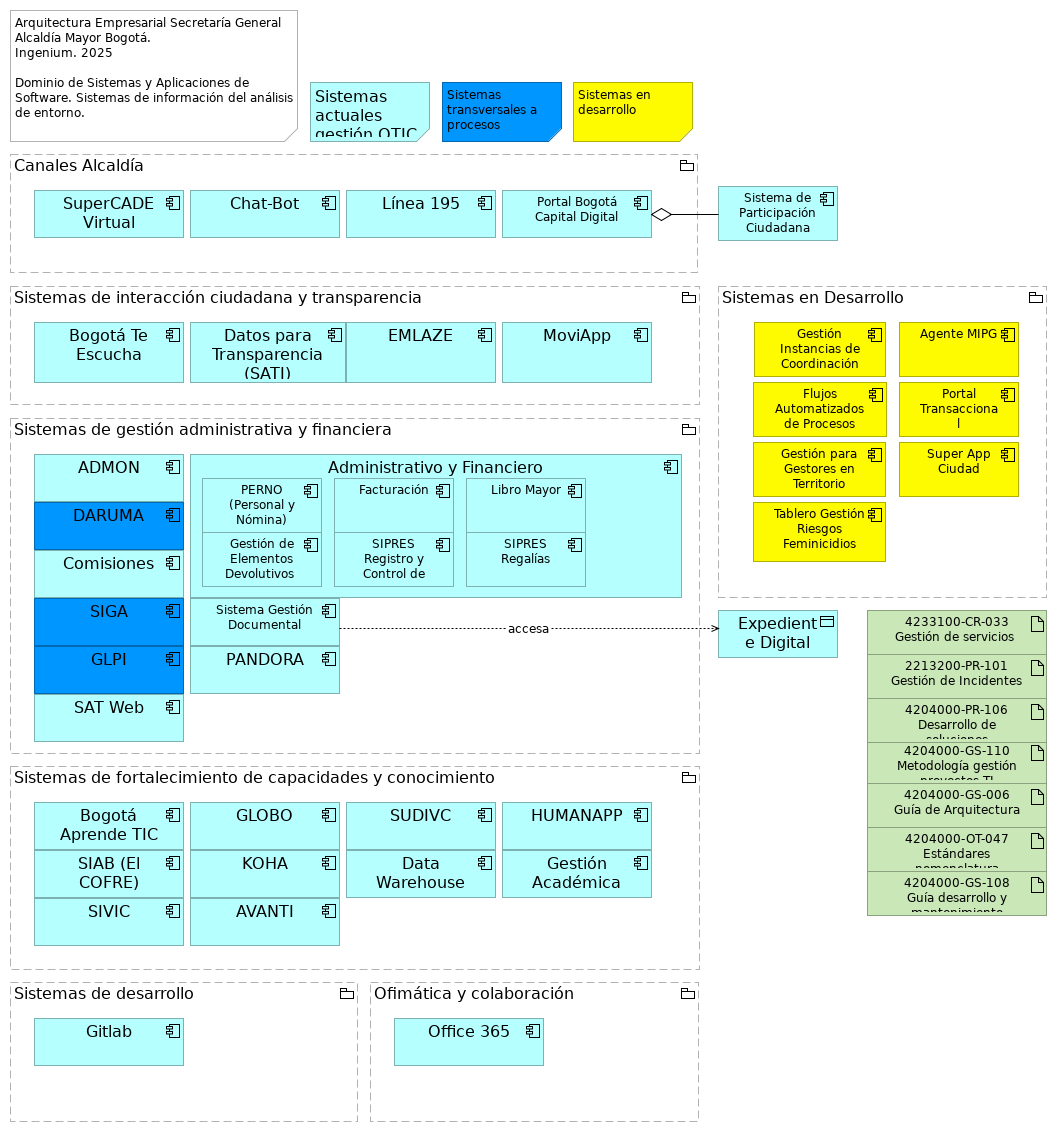
\includegraphics{images/06.2n2.1a.SIdelAnalisisdeEntorno.png}
\caption{06.2n2.1a. SI del Analisis de Entorno. \emph{Fuente: Proyecto
arquitectura empresarial. Arquitectura de Aplicaciones Secretaria
General Alcaldía Mayor de Bogotá
(2025)}}\label{fig:id-097745511d984e7eaf02b5ad5a93e7a8}
\end{figure}

\subsubsection{Elementos del Modelo}\label{sec:elementos-del-modelo}

\begin{longtable}[]{@{}
  >{\raggedright\arraybackslash}p{(\columnwidth - 4\tabcolsep) * \real{0.3000}}
  >{\raggedright\arraybackslash}p{(\columnwidth - 4\tabcolsep) * \real{0.2000}}
  >{\raggedright\arraybackslash}p{(\columnwidth - 4\tabcolsep) * \real{0.5000}}@{}}
\toprule\noalign{}
\begin{minipage}[b]{\linewidth}\raggedright
Nombre
\end{minipage} & \begin{minipage}[b]{\linewidth}\raggedright
Tipo
\end{minipage} & \begin{minipage}[b]{\linewidth}\raggedright
Documentación
\end{minipage} \\
\midrule\noalign{}
\endhead
\bottomrule\noalign{}
\endlastfoot
Canales Alcaldía & Grouping & \\
SuperCADE Virtual & Application Component & Red de canales presenciales
de atención a ciudadanía. \\
& & \\
Chat-Bot & Application Component & Canal web de atención a
ciudadanía. \\
& & \\
Línea 195 & Application Component & Canal telefónico de atención a
ciudadanía. \\
& & \\
Portal Bogotá Capital Digital & Application Component & Plataforma de
Trámites en línea. Portal Integrador de trámites y servicios ofrecidos a
la ciudadanía. Componente de aplicación que permite la realización de
trámites digitales. \\
& & \\
Sistema de Participación Ciudadana & Application Component & Componente
de aplicación para facilitar la interacción y el acercamiento
(realimentación) de los ciudadanos. \\
& & \\
Sistemas de interacción ciudadana y transparencia & Grouping & \\
Bogotá Te Escucha & Application Component & Sistema de información para
la administración, registro, atención, seguimiento y control de las
peticiones, quejas, reclamos, solicitudes de información, denuncias y
sugerencias que reciban las entidades del distrito capital por los
diferentes canales. Fundamental para el proceso de Gobierno abierto y
relacionamiento con la ciudadanía. También se menciona como el Sistema
Distrital para la Gestión de Peticiones Ciudadanas, a través del cual se
evalúa la calidad de las respuestas emitidas a la ciudadanía. \\
& & \\
Datos para Transparencia (SATI) & Application Component & Sistem de
tableros de control con datos relevantes, actualizados y comprensibles,
incluyendo alertas tempranas contra la corrupción. Plataforma que
facilita el acceso a datos e información gubernamental. Soporta el
proceso de Gobierno abierto y relacionamiento con la ciudadanía. \\
& & \\
EMLAZE & Application Component & Sistema para la planeación de recursos
empresariales (ERP) de la Imprenta Distrital y control de ejecución y
consumo de insumos en el ejercicio de imprenta. \\
& & \\
MoviApp & Application Component & Canal móvil de atención a ciudadanía.
Sesión levantamiento no. 2. \\
& & \\
Sistemas en Desarrollo & Grouping & \\
Gestión Instancias de Coordinación & Application Component & Componente
de aplicación para facilitar la interacción y el acercamiento
(realimentación) de los ciudadanos. \\
& & \\
Agente MIPG & Application Component & Componente de aplicación para
facilitar la interacción y el acercamiento (realimentación) de los
ciudadanos. \\
& & \\
Flujos Automatizados de Procesos Empleado con TH y Contratistas &
Application Component & Componente de aplicación para facilitar la
interacción y el acercamiento (realimentación) de los ciudadanos. \\
& & \\
Portal Transaccional & Application Component & Componente de aplicación
para facilitar la interacción y el acercamiento (realimentación) de los
ciudadanos. \\
& & \\
Gestión para Gestores en Territorio & Application Component & Componente
de aplicación para facilitar la interacción y el acercamiento
(realimentación) de los ciudadanos. \\
& & \\
Super App Ciudad & Application Component & Componente de aplicación para
facilitar la interacción y el acercamiento (realimentación) de los
ciudadanos. \\
& & \\
Tablero Gestión Riesgos Feminicidios & Application Component &
Componente de aplicación para facilitar la interacción y el acercamiento
(realimentación) de los ciudadanos. \\
& & \\
Sistemas de gestión administrativa y financiera & Grouping & \\
ADMON & Application Component & Se relaciona con la gestión financiera,
gestión de servicios administrativos y tecnológicos, y gestión de
recursos físicos. \\
& & \\
Administrativo y Financiero & Application Component & Grupo de sistema
de soporte a la gestión financiera, gestión de servicios
administrativos, tecnológicos, y gestión de recursos físicos. \\
& & \\
PERNO (Personal y Nómina) & Application Component & Módulo de Personal y
Nómina (PERNO, heredado de SICAPITAL). \\
& & \\
Facturación & Application Component & Administración de costos y
facturación de los Cades y Supercades (FACTURACIÓN). \\
& & \\
Libro Mayor & Application Component & LIMAY, heredado de SICAPITAL). \\
& & \\
Gestión de Elementos Devolutivos & Application Component & Sistema
control de gestión de elementos devolutivos (SAI, heredado de
SICAPITAL) \\
& & \\
SIPRES Registro y Control de Presupuesto & Application Component &
Registro y control de la información de presupuesto de la Secretaría
General (SIPRES). \\
& & \\
SIPRES Regalías & Application Component & Sistema para manejo y control
del presupuesto de regalías (SIPRES REGALIAS)Registro y control de la
información contractual de la Secretaría General (CONTRACTUAL)Sistema
para manejo de contratos con presupuesto de regalías (CONTRACTUAL
REGALIAS). \\
& & \\
DARUMA & Application Component & Sistema para el registro de documentos
de procesos, procedimientos, formatos, entre otros, como insumos de la
Gestión de Calidad. \\
& & \\
Comisiones & Application Component & Sesión levantamiento no. 1. \\
& & \\
SIGA & Application Component & Sistema Integrado de Gestión Documental,
Archivo y Correspondencia. \\
& & \\
Sistema Gestión Documental & Application Component & Componente de
aplicación para la gestión electrónica de documentos. \\
& & \\
GLPI & Application Component & Sistema de soporta a la gestión de
servicios administrativos y tecnológicos, donde se registran y gestionan
las solicitudes de servicios TIC. \\
& & \\
PANDORA & Application Component & Implementación de temas precontractual
y planeación. \\
& & \\
SAT Web & Application Component & Sistema de Asignación de Turnos en los
puntos de atención a la ciudadanía (Red Cade). \\
& & \\
Expediente Digital & Data Object & Objeto de datos en la capa de
aplicación que representa un expediente electrónico. \\
4233100-CR-033 Gestión de servicios & Artifact & 4233100-CR-033 Gestión
de servicios administrativos y tecnológicos. \\
& & \\
2213200-PR-101 Gestión de Incidentes & Artifact & 2213200-PR-101 Gestión
de Incidentes, Requerimientos y Problemas Tecnológicos. \\
& & \\
4204000-PR-106 Desarrollo de soluciones & Artifact & 4204000-PR-106
Desarrollo de soluciones \\
& & \\
4204000-GS-110 Metodología gestión proyectos TI & Artifact &
4204000-GS-110 Metodología gestión proyectos TI. \\
\end{longtable}

\textbar{} \textbar{} Sistemas de fortalecimiento de capacidades y
conocimiento \textbar{} Grouping \textbar{} \textbar{} \textbar{} Bogotá
Aprende TIC \textbar{} Application Component \textbar{} Portal de apoya
los procesos de Gobierno abierto y relacionamiento con la ciudadanía, y
Fortalecimiento de la Gestión Pública. \textbar{} \textbar{} GLOBO
\textbar{} Application Component \textbar{} Registro de acciones de
cooperación internacional. Utilizado en el proceso de Fortalecimiento de
la Gestión Pública. \textbar{} \textbar{} SUDIVC \textbar{} Application
Component \textbar{} Sistema Unificado Distrital de Inspección,
Vigilancia y Control -- SUDIVC. \textbar{} \textbar{} HUMANAPP
\textbar{} Application Component \textbar{} Apoya la gestión del talento
humano. Aplicativo de generación de desprendibles de pago para
funcionarios y certificaciones laborales, de seguridad social y de
ingresos y retenciones. \textbar{} \textbar{} SIAB (El COFRE) \textbar{}
Application Component \textbar{} Sistema de Información del Archivo de
Bogotá SIAB. Permite automatizar los procesos archivísticos y técnicos
que realiza el Archivo, tales como llevar un registro de los Ingresos
Documentales (antes área de acopio), para la descripción y catalogación
de la documentación, propios del proceso de Gestión de la Función
Archivística y del Patrimonio Documental, para su custodia y
conservación permanente. Utilizado en los procesos de Gobierno abierto y
relacionamiento con la ciudadanía, y Fortalecimiento de la Gestión
Pública. \textbar{} \textbar{} KOHA \textbar{} Application Component
\textbar{} Sistema Integrado de Gestión de Bibliotecas. Relacionado con
la Gestión del conocimiento. \textbar{} \textbar{} Data Warehouse
\textbar{} Application Component \textbar{} Almacenes de datos de
trabajo de SG. Bodega de datos con diversas fuentes de información para
el análisis y transformación de datos de interés. \textbar{} \textbar{}
Gestión Académica \textbar{} Application Component \textbar{} Moodle
para capacitación de servidores de la Entidad en diferentes temas.
Relacionado con la Gestión del conocimiento. \textbar{} \textbar{} SIVIC
\textbar{} Application Component \textbar{} Sistema de Información de
Víctimas de Bogotá para registrar la gestión de atención integral a las
víctimas. Interviene en los procesos de Paz, víctimas y reconciliación,
y Fortalecimiento de la Gestión Pública. Interviene en los procesos de
Paz, víctimas y reconciliación, y Fortalecimiento de la Gestión Pública.
\textbar{} \textbar{} AVANTI \textbar{} Application Component \textbar{}
Sistema de Información para registrar avance de programación y
seguimiento de metas plan de desarrollo de las entidades distritales
SDARIV relacionadas con atención integral a las víctimas. \textbar{}
\textbar{} 4204000-GS-006 Guía de Arquitectura \textbar{} Artifact
\textbar{} 4204000-GS-006 Guía de Arquitectura de Software para
Soluciones Tecnológicas. \textbar{} \textbar{} 4204000-OT-047 Estándares
nomenclatura \textbar{} Artifact \textbar{} 4204000-OT-047 Estándares de
nomenclatura para el desarrollo de aplicaciones en ambientes de bases de
datos. \textbar{} \textbar{} 4204000-GS-108 Guía desarrollo y
mantenimiento \textbar{} Artifact \textbar{} 4204000-GS-108 Guía
Metodológica para el desarrollo y mantenimiento de soluciones de
software \textbar{} \textbar{} Sistemas de desarrollo \textbar{}
Grouping \textbar{} \textbar{} \textbar{} Gitlab \textbar{} Application
Component \textbar{} Plataforma de desarrollo de software y
colaboración. \textbar{} \textbar{} Ofimática y colaboración \textbar{}
Grouping \textbar{} \textbar{} \textbar{} Office 365 \textbar{}
Application Component \textbar{} Herramientas de ofimática y
colaboración SG. \textbar{}

Table: Elementos de la vista.
\{\#tbl:tblelement-06.2n2.1a.SIdelAnalisisdeEntorno-id\}

\subsection{Alineación de aplicaciones de software con los procesos
SG}\label{sec:alineaciuxf3n-de-aplicaciones-de-software-con-los-procesos-sg}

\begin{quote}
\end{quote}

La Secretaría General cuenta con sistemas de información que soportan
las actividades gestionadas por los procesos misionales, estratégicos,
de apoyo y de evaluación y control. Del análisis de fuentes y
levantamientos de información presentamos la alineación entre las
aplicaciones de software de SG, los procesos de negocio y el estado
actual.

\begin{longtable}[]{@{}
  >{\raggedright\arraybackslash}p{(\columnwidth - 4\tabcolsep) * \real{0.2045}}
  >{\raggedright\arraybackslash}p{(\columnwidth - 4\tabcolsep) * \real{0.2992}}
  >{\raggedright\arraybackslash}p{(\columnwidth - 4\tabcolsep) * \real{0.4962}}@{}}
\toprule\noalign{}
\begin{minipage}[b]{\linewidth}\raggedright
Proceso
\end{minipage} & \begin{minipage}[b]{\linewidth}\raggedright
Sistema de Información
\end{minipage} & \begin{minipage}[b]{\linewidth}\raggedright
Oportunidad de Mejora
\end{minipage} \\
\midrule\noalign{}
\endhead
\bottomrule\noalign{}
\endlastfoot
Control Disciplinario & Gestión Documental - SIGA & Actualización de la
versión de la aplicación y su infraestructura \\
Evaluación del Sistema de Control Interno & Gestión Documental - SIGA &
Actualización de la versión de la aplicación y su infraestructura \\
Gestión Jurídica & Gestión Documental - SIGA & Actualización de la
versión de la aplicación y su infraestructura \\
Gestión de contratación & Administrativo y Financiero (Gestión
Contractual) & Actualización tecnológica para optimizar el rendimiento y
acceso al sistema de información y atención de requerimientos a
demanda \\
Gestión Financiera & Administrativo y Financiero (Facturación, LIMAY,
Gestión Contractual, SIPRES) & Actualización tecnológica para optimizar
el rendimiento y acceso al sistema de información y atención de
requerimientos a demanda \\
Gestión de servicios administrativos y tecnológicos & GitLab, GLPI &
Atención de requerimientos a demanda \\
Gestión de servicios administrativos y tecnológicos & Administrativo y
Financiero (Inventario, SAI, SAE, Control de vehículos) & Actualización
tecnológica para optimizar el rendimiento y acceso al sistema de
información y atención de requerimientos a demanda \\
Gestión de recursos físicos & Administrativo y Financiero (Inventario,
SAI SAE, Control de vehículos) & Actualización tecnológica para
optimizar el rendimiento y acceso al sistema de información y atención
de requerimientos a demanda \\
Gestión del Talento Humano & Administrativo y Financiero (PERNO) &
Actualización tecnológica para optimizar el rendimiento y acceso al
sistema de información y atención de requerimientos a demanda \\
Gestión del Talento Humano & HUMANAPP & Actualización tecnológica para
optimizar el rendimiento y acceso al sistema de información y atención
de requerimientos a demanda \\
Gobierno abierto y relacionamiento con la ciudadanía & Bogotá Te Escucha
& Actualización de la versión de la aplicación y su infraestructura \\
Gobierno abierto y relacionamiento con la ciudadanía & Data Warehouse &
Vincular más Fuentes de información \\
Gobierno abierto y relacionamiento con la ciudadanía & SAT Web &
Actualización de su infraestructura \\
Gobierno abierto y relacionamiento con la ciudadanía & SUDIVC & Atención
de requerimientos a demanda \\
Paz, víctimas y reconciliación & SIVIC & Atención de requerimientos a
demanda \\
Paz, víctimas y reconciliación & AVANTI & Atención de requerimientos a
demanda \\
Fortalecimiento de la Gestión Pública & SIAB (Cofre) & Atención de
requerimientos a demanda \\
Fortalecimiento de la Gestión Pública & KOHA & Atención de
requerimientos a demanda \\
Fortalecimiento de la Gestión Pública & Datos para la transparencia
(SATI) & Atención de requerimientos a demanda \\
Fortalecimiento de la Gestión Pública & EMLAZE & Atención de
requerimientos a demanda y con proveedor externo para el caso de
Emlaze \\
Direccionamiento Estratégico & DARUMA & Atención de requerimientos a
demanda con proveedor externo \\
Gestión estratégica de comunicación e información & Gestión Documental -
SIGA & Actualización de la versión de la aplicación y su
infraestructura \\
Fortalecimiento Institucional & Gestión académica & Atención de
requerimientos a demanda \\
Gestión de alianzas e internacionalización de Bogotá & Globo & Atención
de requerimientos a demanda \\
Gestión del conocimiento & Bogotá Aprende TIC & Atención de
requerimientos a demanda \\
\end{longtable}

Es importante destacar que el sistema Integrado de Gestión de Calidad
DARUMA, el Sistema de Gestión de Incidentes y Solicitudes GLPI, y el
Sistema de Gestión Documental SIGA, son sistemas transversales que
soportan todos los procesos de la Secretaría General de la Alcaldía
Mayor de Bogotá D.C..

\begin{figure}
\centering
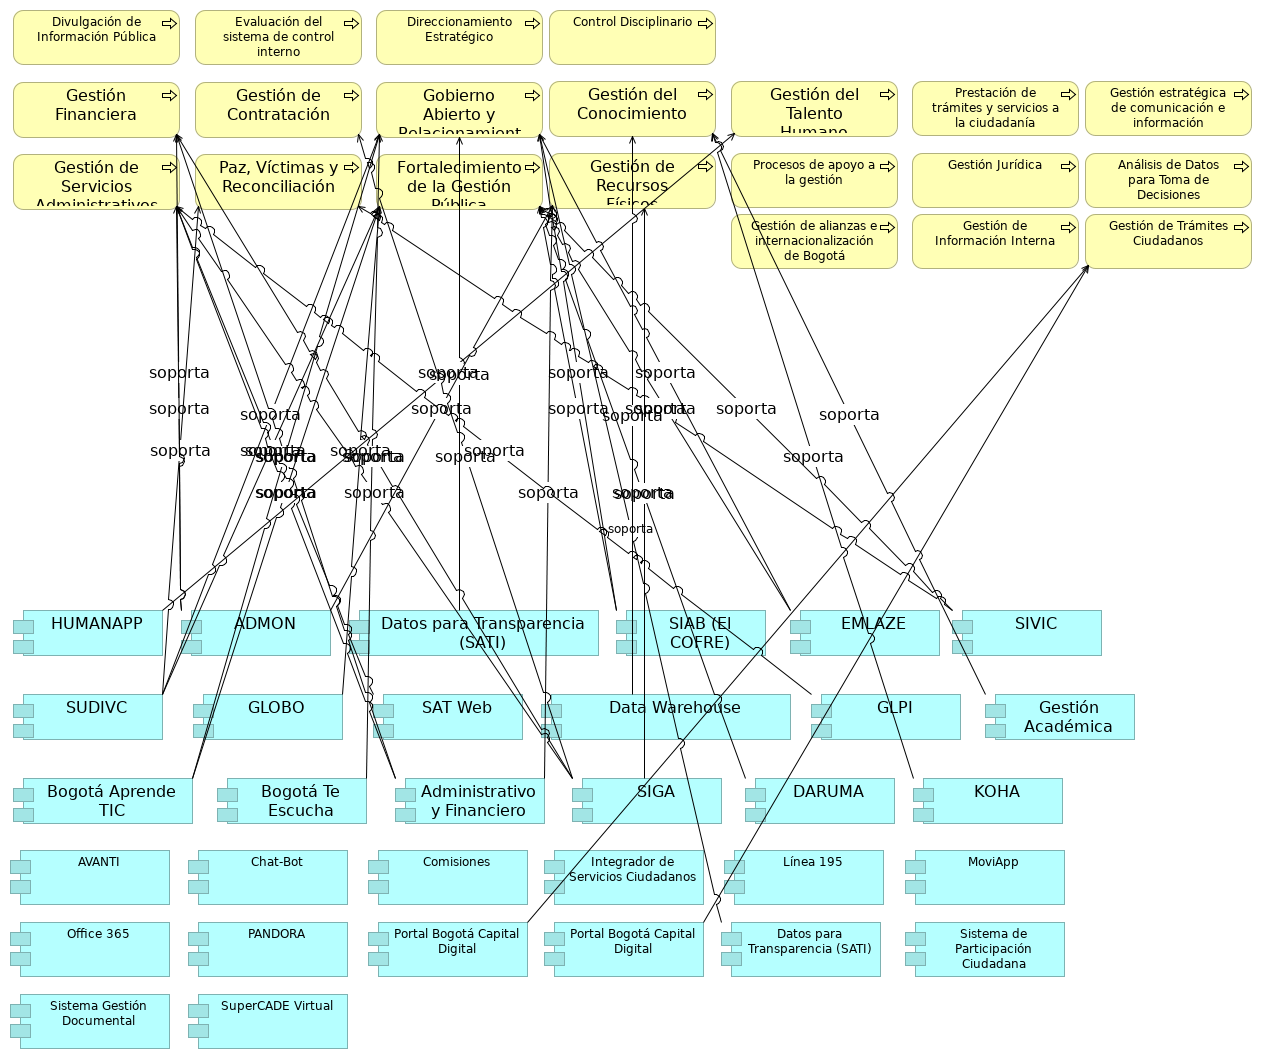
\includegraphics{images/06.2n3.a.AplicacionesyProcesos.png}
\caption{06.2n3.a. Aplicaciones y Procesos. \emph{Fuente: Proyecto
arquitectura empresarial. Arquitectura de Aplicaciones Secretaria
General Alcaldía Mayor de Bogotá
(2025)}}\label{fig:id-7812cd6a3a0d4d5783b00f16f2c5826b}
\end{figure}

\subsubsection{Divulgación de Información
Pública}\label{sec:divulgaciuxf3n-de-informaciuxf3n-puxfablica}

Proceso de negocio para la difusión optimizada de información a través
de sistemas digitales.

\subsubsection{Evaluación del sistema de control
interno}\label{sec:evaluaciuxf3n-del-sistema-de-control-interno}

Evaluar de manera independiente y objetiva el Sistema de Control Interno
de la Secretaría General de la Alcaldía Mayor de Bogotá, mediante la
realización de auditorías internas de gestión, seguimientos e informes
regulatorios programados en el Plan de Anual de Auditorías, y la
atención a organismos de control, con el propósito de contribuir al
mejoramiento continuo de la gestión institucional.

\subsubsection{Direccionamiento
Estratégico}\label{sec:direccionamiento-estratuxe9gico}

Formular, implementar, hacer monitoreo y seguimiento a las políticas
públicas competencia de la Secretaría General, a los planes
institucionales, a los proyectos de inversión, y gestionar el
presupuesto de inversión mediante la definición de orientaciones,
metodologías, la retroalimentación, acompañamiento y articulación a las
dependencias de la entidad con el fin de cumplir el logro de la misión y
los objetivos institucionales, en el marco de una cultura de
transparencia.

\subsubsection{Control Disciplinario}\label{sec:control-disciplinario}

Adelantar los procesos disciplinarios contra los(as) servidores(as) y
exservidores(as) de la Secretaría General de la Alcaldía Mayor de Bogotá
D.C., y prevenir las conductas disciplinarias mediante la aplicación de
las normas vigentes en materia disciplinaria y el desarrollo de la
estrategia preventiva con el fin determinar la posible responsabilidad
disciplinaria, y evitar la ocurrencia de faltas disciplinarias por parte
de estos.

\subsubsection{Gestión del
Conocimiento}\label{sec:gestiuxf3n-del-conocimiento}

Gestionar el conocimiento y la innovación de la Secretaría General de la
Alcaldía Mayor de Bogotá, mediante la identificación, generación,
sistematización, análisis, transferencia y conservación del conocimiento
estratégico y la promoción de la innovación, con el fin de fortalecer el
aprendizaje, el mejoramiento organizacional y la toma de decisiones
basada en evidencias.

\subsubsection{Gestión del Talento
Humano}\label{sec:gestiuxf3n-del-talento-humano}

Gestionar el capital humano de la Secretaría General, y vincular y
administrar el Gabinete distrital y jefatura del talento humano interno
mediante el Plan Estratégico de Talento Humano para la Secretaría
General y el trámite de situaciones administrativas con el fin de
fortalecer el sentido de pertenencia y contribuir a la calidad de vida
del talento humano de la entidad.

\subsubsection{Prestación de trámites y servicios a la
ciudadanía}\label{sec:prestaciuxf3n-de-truxe1mites-y-servicios-a-la-ciudadanuxeda}

Proceso central para la interacción con los ciudadanos.

\subsubsection{Gestión estratégica de comunicación e
información}\label{sec:gestiuxf3n-estratuxe9gica-de-comunicaciuxf3n-e-informaciuxf3n}

Mantener informados a los distintos grupos de valor e interés acerca de
los programas, proyectos y gestión de la Administración Distrital a
través de la formulación y la implementación de estrategias de
comunicación pública con el propósito de interactuar y mantener la
confianza por parte de la entidad y de la ciudadanía en general.

\subsubsection{Gestión Financiera}\label{sec:gestiuxf3n-financiera}

Gestionar las operaciones financieras con cargo al presupuesto asignado
a la entidad, a través del registro de las operaciones económicas en
contabilidad para garantizar la elaboración y reporte de los estados
financieros a los entes de control en forma comprensible, relevante y
confiable, para que sean consultados por los ciudadanos y por los
interesados en la información financiera.

\subsubsection{Gestión de
Contratación}\label{sec:gestiuxf3n-de-contrataciuxf3n}

Gestionar la contratación de bienes, servicios y obras, mediante el
desarrollo de procesos contractuales transparentes y conforme a la
normativa legal vigente para satisfacer las necesidades de contratación
de las dependencias de la Secretaría General de la Alcaldía Mayor de
Bogotá, y contribuir al cumplimento de sus metas y objetivos.

\subsubsection{Gobierno Abierto y Relacionamiento con la
Ciudadanía}\label{sec:gobierno-abierto-y-relacionamiento-con-la-ciudadanuxeda}

Fortalecer relación entre la administración distrital y la ciudadanía
mediante la formulación de lineamientos, desarrollo de estrategias y
proyectos, fortalecimiento de capacidades, seguimiento y evaluación en
materia de servicio a la ciudadanía, gobierno abierto y transformación
digital de la Secretaría General y de las entidades distritales, para el
acceso oportuno, efectivo y de calidad a la oferta institucional de
bienes y servicios.

\subsubsection{Gestión de Recursos
Físicos}\label{sec:gestiuxf3n-de-recursos-fuxedsicos}

Administrar los bienes que legalmente están a cargo de la Secretaría
General de la Alcaldía Mayor de Bogotá D.C. mediante su recepción,
asignación, mantenimiento, control, baja y/o destinación final con el
fin de cubrir las necesidades de recursos físicos de las dependencias.

\subsubsection{Procesos de apoyo a la
gestión}\label{sec:procesos-de-apoyo-a-la-gestiuxf3n}

Procesos internos que facilitan la operación de la entidad.

\subsubsection{Gestión Jurídica}\label{sec:gestiuxf3n-juruxeddica}

Asesorar y representar jurídicamente a la Secretaría General de la
Alcaldía Mayor Bogotá D.C. mediante el análisis, trámite, defensa,
solución y respuesta de asuntos de carácter jurídico que surjan en el
desarrollo de las funciones de acuerdo con la normatividad vigente.

\subsubsection{Análisis de Datos para Toma de
Decisiones}\label{sec:anuxe1lisis-de-datos-para-toma-de-decisiones}

Proceso de negocio que utiliza software especializado para el análisis
de datos.

\subsubsection{Gestión de Servicios Administrativos y
Tecnológicos}\label{sec:gestiuxf3n-de-servicios-administrativos-y-tecnoluxf3gicos}

Apoyar la gestión de la Entidad a través de la prestación de los
servicios administrativos y tecnológicos, así como, de la gestión
documental, con el fin de satisfacer las necesidades de las dependencias
en la materia, al igual que conservar y preservar la memoria
institucional.

\subsubsection{Paz, Víctimas y
Reconciliación}\label{sec:paz-vuxedctimas-y-reconciliaciuxf3n}

Gestionar políticas, programas y estrategias dirigidas a las víctimas,
población en proceso de reintegración, reincorporación, comparecientes
de fuerza pública y ciudadanía en general por medio de la asistencia,
atención, reparación, y acciones de memoria, reconciliación y
construcción de paz territorial con el propósito de que Bogotá sea un
territorio de paz y reconciliación, donde todos puedan volver a empezar.

\subsubsection{Fortalecimiento de la Gestión
Pública}\label{sec:fortalecimiento-de-la-gestiuxf3n-puxfablica}

Generar capacidades institucionales en las entidades distritales a
través del desarrollo de estudios, investigaciones y estrategias
relacionadas con el fortalecimiento de la gestión, impresión de artes
gráficas y la publicación de la Gaceta Pública en el registro distrital;
con el fin, de modernizar y mejorar el desempeño de la administración
distrital.

\subsubsection{Gestión de alianzas e internacionalización de
Bogotá}\label{sec:gestiuxf3n-de-alianzas-e-internacionalizaciuxf3n-de-bogotuxe1}

Facilitar acciones estratégicas de cooperación, relacionamiento y
posicionamiento internacional, mediante la gestión de interacciones con
actores nacionales e internacionales, con el fin de movilizar recursos
técnicos y financieros, generar alianzas estratégicas y posicionar a
Bogotá como un referente global. De esta manera, se contribuirá a la
implementación del Plan de Desarrollo Distrital, fortalecerá las
políticas públicas y la gestión del Distrito, y se alineará con
iniciativas globales como la Agenda 2030.

\subsubsection{Gestión de Información
Interna}\label{sec:gestiuxf3n-de-informaciuxf3n-interna}

Proceso de recolección, procesamiento y distribución de información
dentro de la entidad.

\subsubsection{Gestión de Trámites
Ciudadanos}\label{sec:gestiuxf3n-de-truxe1mites-ciudadanos}

Proceso de atención y resolución de solicitudes y gestiones de los
ciudadanos.

\subsubsection{HUMANAPP}\label{sec:humanapp}

Apoya la gestión del talento humano. Aplicativo de generación de
desprendibles de pago para funcionarios y certificaciones laborales, de
seguridad social y de ingresos y retenciones.

\subsubsection{ADMON}\label{sec:admon}

Se relaciona con la gestión financiera, gestión de servicios
administrativos y tecnológicos, y gestión de recursos físicos.

\subsubsection{Datos para Transparencia
(SATI)}\label{sec:datos-para-transparencia-sati}

Sistem de tableros de control con datos relevantes, actualizados y
comprensibles, incluyendo alertas tempranas contra la corrupción.
Plataforma que facilita el acceso a datos e información gubernamental.
Soporta el proceso de Gobierno abierto y relacionamiento con la
ciudadanía.

\subsubsection{SIAB (El COFRE)}\label{sec:siab-el-cofre}

Sistema de Información del Archivo de Bogotá SIAB. Permite automatizar
los procesos archivísticos y técnicos que realiza el Archivo, tales como
llevar un registro de los Ingresos Documentales (antes área de acopio),
para la descripción y catalogación de la documentación, propios del
proceso de Gestión de la Función Archivística y del Patrimonio
Documental, para su custodia y conservación permanente. Utilizado en los
procesos de Gobierno abierto y relacionamiento con la ciudadanía, y
Fortalecimiento de la Gestión Pública.

\subsubsection{EMLAZE}\label{sec:emlaze}

Sistema para la planeación de recursos empresariales (ERP) de la
Imprenta Distrital y control de ejecución y consumo de insumos en el
ejercicio de imprenta.

\subsubsection{SIVIC}\label{sec:sivic}

Sistema de Información de Víctimas de Bogotá para registrar la gestión
de atención integral a las víctimas. Interviene en los procesos de Paz,
víctimas y reconciliación, y Fortalecimiento de la Gestión Pública.
Interviene en los procesos de Paz, víctimas y reconciliación, y
Fortalecimiento de la Gestión Pública.

\subsubsection{SUDIVC}\label{sec:sudivc}

Sistema Unificado Distrital de Inspección, Vigilancia y Control --
SUDIVC.

\subsubsection{GLOBO}\label{sec:globo}

Registro de acciones de cooperación internacional. Utilizado en el
proceso de Fortalecimiento de la Gestión Pública.

\subsubsection{SAT Web}\label{sec:sat-web}

Sistema de Asignación de Turnos en los puntos de atención a la
ciudadanía (Red Cade).

\subsubsection{Data Warehouse}\label{sec:data-warehouse}

Almacenes de datos de trabajo de SG. Bodega de datos con diversas
fuentes de información para el análisis y transformación de datos de
interés.

\subsubsection{GLPI}\label{sec:glpi}

Sistema de soporta a la gestión de servicios administrativos y
tecnológicos, donde se registran y gestionan las solicitudes de
servicios TIC.

\subsubsection{Gestión Académica}\label{sec:gestiuxf3n-acaduxe9mica}

Moodle para capacitación de servidores de la Entidad en diferentes
temas. Relacionado con la Gestión del conocimiento.

\subsubsection{Bogotá Aprende TIC}\label{sec:bogotuxe1-aprende-tic}

Portal de apoya los procesos de Gobierno abierto y relacionamiento con
la ciudadanía, y Fortalecimiento de la Gestión Pública.

\subsubsection{Bogotá Te Escucha}\label{sec:bogotuxe1-te-escucha}

Sistema de información para la administración, registro, atención,
seguimiento y control de las peticiones, quejas, reclamos, solicitudes
de información, denuncias y sugerencias que reciban las entidades del
distrito capital por los diferentes canales. Fundamental para el proceso
de Gobierno abierto y relacionamiento con la ciudadanía. También se
menciona como el Sistema Distrital para la Gestión de Peticiones
Ciudadanas, a través del cual se evalúa la calidad de las respuestas
emitidas a la ciudadanía.

\subsubsection{Administrativo y
Financiero}\label{sec:administrativo-y-financiero}

Grupo de sistema de soporte a la gestión financiera, gestión de
servicios administrativos, tecnológicos, y gestión de recursos físicos.

\subsubsection{SIGA}\label{sec:siga}

Sistema Integrado de Gestión Documental, Archivo y Correspondencia.

\subsubsection{DARUMA}\label{sec:daruma}

Sistema para el registro de documentos de procesos, procedimientos,
formatos, entre otros, como insumos de la Gestión de Calidad.

\subsubsection{KOHA}\label{sec:koha}

Sistema Integrado de Gestión de Bibliotecas. Relacionado con la Gestión
del conocimiento.

\subsubsection{AVANTI}\label{sec:avanti}

Sistema de Información para registrar avance de programación y
seguimiento de metas plan de desarrollo de las entidades distritales
SDARIV relacionadas con atención integral a las víctimas.

\subsubsection{Chat-Bot}\label{sec:chat-bot}

Canal web de atención a ciudadanía.

\subsubsection{Comisiones}\label{sec:comisiones}

Sesión levantamiento no. 1.

\subsubsection{Integrador de Servicios
Ciudadanos}\label{sec:integrador-de-servicios-ciudadanos}

Plataforma unificada para acceder a servicios y trámites ciudadanos.

\subsubsection{Línea 195}\label{sec:luxednea-195}

Canal telefónico de atención a ciudadanía.

\subsubsection{MoviApp}\label{sec:moviapp}

Canal móvil de atención a ciudadanía. Sesión levantamiento no. 2.

\subsubsection{Office 365}\label{sec:office-365}

Herramientas de ofimática y colaboración SG.

\subsubsection{PANDORA}\label{sec:pandora}

Implementación de temas precontractual y planeación.

\subsubsection{Portal Bogotá Capital
Digital}\label{sec:portal-bogotuxe1-capital-digital}

Plataforma de Trámites en línea. Portal Integrador de trámites y
servicios ofrecidos a la ciudadanía. Componente de aplicación que
permite la realización de trámites digitales.

\subsubsection{Portal Bogotá Capital
Digital}\label{sec:portal-bogotuxe1-capital-digital-1}

Plataforma de Trámites en línea. Portal Integrador de trámites y
servicios ofrecidos a la ciudadanía. Componente de aplicación que
permite la realización de trámites digitales.

\subsubsection{Datos para Transparencia
(SATI)}\label{sec:datos-para-transparencia-sati-1}

Sistem de tableros de control con datos relevantes, actualizados y
comprensibles, incluyendo alertas tempranas contra la corrupción.
Plataforma que facilita el acceso a datos e información gubernamental.
Soporta el proceso de Gobierno abierto y relacionamiento con la
ciudadanía.

\subsubsection{Sistema de Participación
Ciudadana}\label{sec:sistema-de-participaciuxf3n-ciudadana}

Componente de aplicación para facilitar la interacción y el acercamiento
(realimentación) de los ciudadanos.

\subsubsection{Sistema Gestión
Documental}\label{sec:sistema-gestiuxf3n-documental}

Componente de aplicación para la gestión electrónica de documentos.

\subsubsection{SuperCADE Virtual}\label{sec:supercade-virtual}

Red de canales presenciales de atención a
ciudadanía.\sidenote{This is a sidenote. This template features a large margin specifically so you can put notes, figures, tables and other things into it as additional material to the main content in the text block.}

Donec in elit ac ante vestibulum rhoncus. Pellentesque ligula tortor, aliquet malesuada nulla tristique vitae. Aliquam mi sem, varius eu pellentesque et, tristique nec quam. Vestibulum pellentesque in dui et venenatis. Sed malesuada elit pellentesque sapien aliquet porta. In at facilisis diam. Duis id ante tellus.\sidenote[][2cm]{This sidenote has been pushed down the page manually with an optional parameter, otherwise it would be right under the one above.} % This first optional argument to a sidenote is the symbol to use (leave this empty for automatic numbering) and the second is the vertical offset (positive is down, negative is up)

In diam libero, vulputate quis accumsan non, auctor in ipsum. Praesent cursus velit eget lacus sodales porta. Proin quis risus ut velit euismod scelerisque ut sed neque. Cras sagittis, dolor ac ullamcorper auctor, tortor dui facilisis diam, at sagittis nisi ipsum a neque. Nullam vel mattis nisi. Ut interdum ut diam at ornare. Nulla ultrices elit justo, vitae tristique massa vulputate sit amet.

\nonumsidenote{
	}Vestibulum erat felis, cursus vitae convallis ac, commodo eu nisi. Nulla facilisi. Mauris dignissim nisi felis, a mollis ex accumsan vel. Suspendisse bibendum vitae nibh in suscipit. Vestibulum et finibus eros. Nulla facilisi. Cras luctus aliquam finibus. In nec justo nec orci malesuada faucibus.

\subsubsection{Subsubsection Title} % Third level section

\begin{fullwidth} % Use the whole page width
	\textit{This is an example of a full width paragraph\ldots} Curabitur id placerat orci. Vivamus pulvinar augue ac feugiat blandit. Donec in ultricies mi. Nam eu lacus ac augue aliquet consectetur. Praesent dui risus, sollicitudin nec felis ut, posuere ultricies dolor. Sed massa nulla, dignissim eget sem sit amet, eleifend fermentum dui. Phasellus consequat sem vel turpis finibus, a aliquam risus malesuada.
\end{fullwidth}

Maecenas consectetur metus at tellus finibus condimentum. Proin arcu lectus, ultrices non tincidunt et, tincidunt ut quam. Integer luctus posuere est, non maximus ante dignissim quis. Nunc a cursus erat. Curabitur suscipit nibh in tincidunt sagittis. Nam malesuada vestibulum quam id gravida. Proin ut dapibus velit. Vestibulum eget quam quis ipsum semper convallis. Duis consectetur nibh ac diam dignissim, id condimentum enim dictum. Nam aliquet ligula eu magna pellentesque, nec sagittis leo lobortis. Aenean tincidunt dignissim egestas. Morbi efficitur risus ante, id tincidunt odio pulvinar vitae.

\paragraph{Paragraph Title} % Fourth level section

Lorem ipsum dolor sit amet, consectetur adipiscing elit. Aliquam auctor mi risus, quis tempor libero hendrerit at. Duis hendrerit placerat quam et semper. Nam ultricies metus vehicula arcu viverra, vel ullamcorper justo elementum. Pellentesque vel mi ac lectus cursus posuere et nec ex.

The section titles below show how multi-line section titles look at the 3 top levels.


%----------------------------------------------------------------------------------------
%	QUOTATIONS
%----------------------------------------------------------------------------------------

\section{Quotations}

Proin mollis urna posuere fringilla. Curabitur finibus, neque vitae vestibulum vestibulum, dolor sapien tincidunt augue, vel porta mauris metus nec mauris. Integer erat magna, porta id erat sed, lacinia volutpat erat. Nulla fermentum tellus arcu, eu iaculis ipsum malesuada aliquam. Duis et lacus maximus, consectetur metus et, eleifend arcu. Vestibulum condimentum diam vitae diam tincidunt viverra.\sidenotequote[-1cm]{\textbf{\LARGE ``}Lorem ipsum dolor sit amet, consectetur adipiscing elit. Praesent porttitor arcu luctus, imperdiet urna iaculis, mattis eros. Pellentesque iaculis odio vel nisl ullamcorper, nec faucibus ipsum molestie.\textbf{''}\\[4pt]\hfill--- John Smith, 1972} % Example margin quotation using the \sidenotequote custom command

\begin{quote}
	\textbf{\LARGE ``}Lorem ipsum dolor sit amet, consectetur adipiscing elit. Praesent porttitor arcu luctus, imperdiet urna iaculis, mattis eros. Pellentesque iaculis odio vel nisl ullamcorper, nec faucibus ipsum molestie. Sed dictum nisl non aliquet porttitor. Etiam vulputate arcu dignissim, finibus sem et, viverra nisl. Aenean luctus congue massa, ut laoreet metus ornare in.\textbf{''}
	
	\hfill--- John Smith, 1972
\end{quote}

Suspendisse tempus odio sit amet volutpat suscipit. Pellentesque ornare libero lacus, non fringilla dolor placerat in. Ut maximus ullamcorper lectus, a pharetra mi sagittis aliquet. Scelerisque augue sed mi fringilla, vel dapibus ligula finibus. Sed ornare velit sem, ac venenatis velit dignissim. Vestibulum ultrices mi at tincidunt condimentum.

%----------------------------------------------------------------------------------------
%	TABLES
%----------------------------------------------------------------------------------------

\section{Table Examples}

This statement automatically references the table below using its label: Table \ref{tab:example}.

%------------------------------------------------

\begin{margintable} % Use the margintable environment for tables to be output to the margin
	\footnotesize % Reduce the font size in the table as space is at a premium
	\caption{Margin table caption.}
	\begin{tabular}{L{0.22\linewidth} C{0.22\linewidth} R{0.25\linewidth}}
		\toprule
		\textbf{Year} & \textbf{Qtr.} & \textbf{Perf.}\\
		\midrule
		20XX & Q1 & 0.5\%\\
		20XX & Q2 & 26.5\%\\
		20XX & Q1 & 35.4\%\\
		20XX & Q4 & 41.3\%\\
		\bottomrule
	\end{tabular}
\end{margintable}

%------------------------------------------------

\begin{table}[H] % [H] forces the table to be output where it is defined in the code (it suppresses floating)
	\caption{Text block table caption.}
	\begin{tabular}{L{0.35\linewidth} L{0.38\linewidth} L{0.16\linewidth}}
		\toprule
		\textbf{Prospect} & \textbf{Industry} & \textbf{Revenue} \\
		\midrule
		Gerlach Inc & Business Development & 3M\\
		Doyle and Sons & Law & 1M\\
		Heathcote Group & Consulting & 12M\\
		Goyette Inc & Advertising & 5M\\
		Holzdeppe GmbH & Manufacturing & 23M\\
		Bienias AG & Accounting & 2.5M\\
		\bottomrule
	\end{tabular}
	\label{tab:example}
\end{table}

%------------------------------------------------

\begin{table*} % Use the table* environment for full width tables
	\caption{Full width table caption.}
	\begin{tabular}{C{0.03\linewidth} L{0.25\linewidth} L{0.27\linewidth} L{0.16\linewidth} L{0.16\linewidth}}
		\toprule
		\textit{\#} & \textbf{Prospect} & \textbf{Industry} & \textbf{Revenue} & \textbf{Employees} \\
		\midrule
		\textit{1} & Gerlach Inc & Business Development & 3M & 65\\
		\textit{2} & Doyle and Sons & Law & 1M & 15\\
		\textit{3} & Heathcote Group & Consulting & 12M & 250\\
		\textit{4} & Goyette Inc & Advertising & 5M & 100\\
		\textit{5} & Holzdeppe GmbH & Manufacturing & 23M & 75\\
		\textit{6} & Bienias AG & Accounting & 2.5M & 40\\
		\bottomrule
	\end{tabular}
\end{table*}

%----------------------------------------------------------------------
%	FIGURES
%----------------------------------------------------------------------

\section{Figure Examples}

This statement automatically references the figure below using its label: Figure \ref{fig:example}.

%------------------------------------------------

\begin{marginfigure} % Use the marginfigure environment for figures to be output to the margin
	
\includegraphics[width=\linewidth]{./include/placeholder.jpg}
	\caption{Margin figure caption.}
\end{marginfigure}

%------------------------------------------------

\begin{figure}[H] % [H] forces the figure to be output where it is defined in the code (it suppresses floating)
	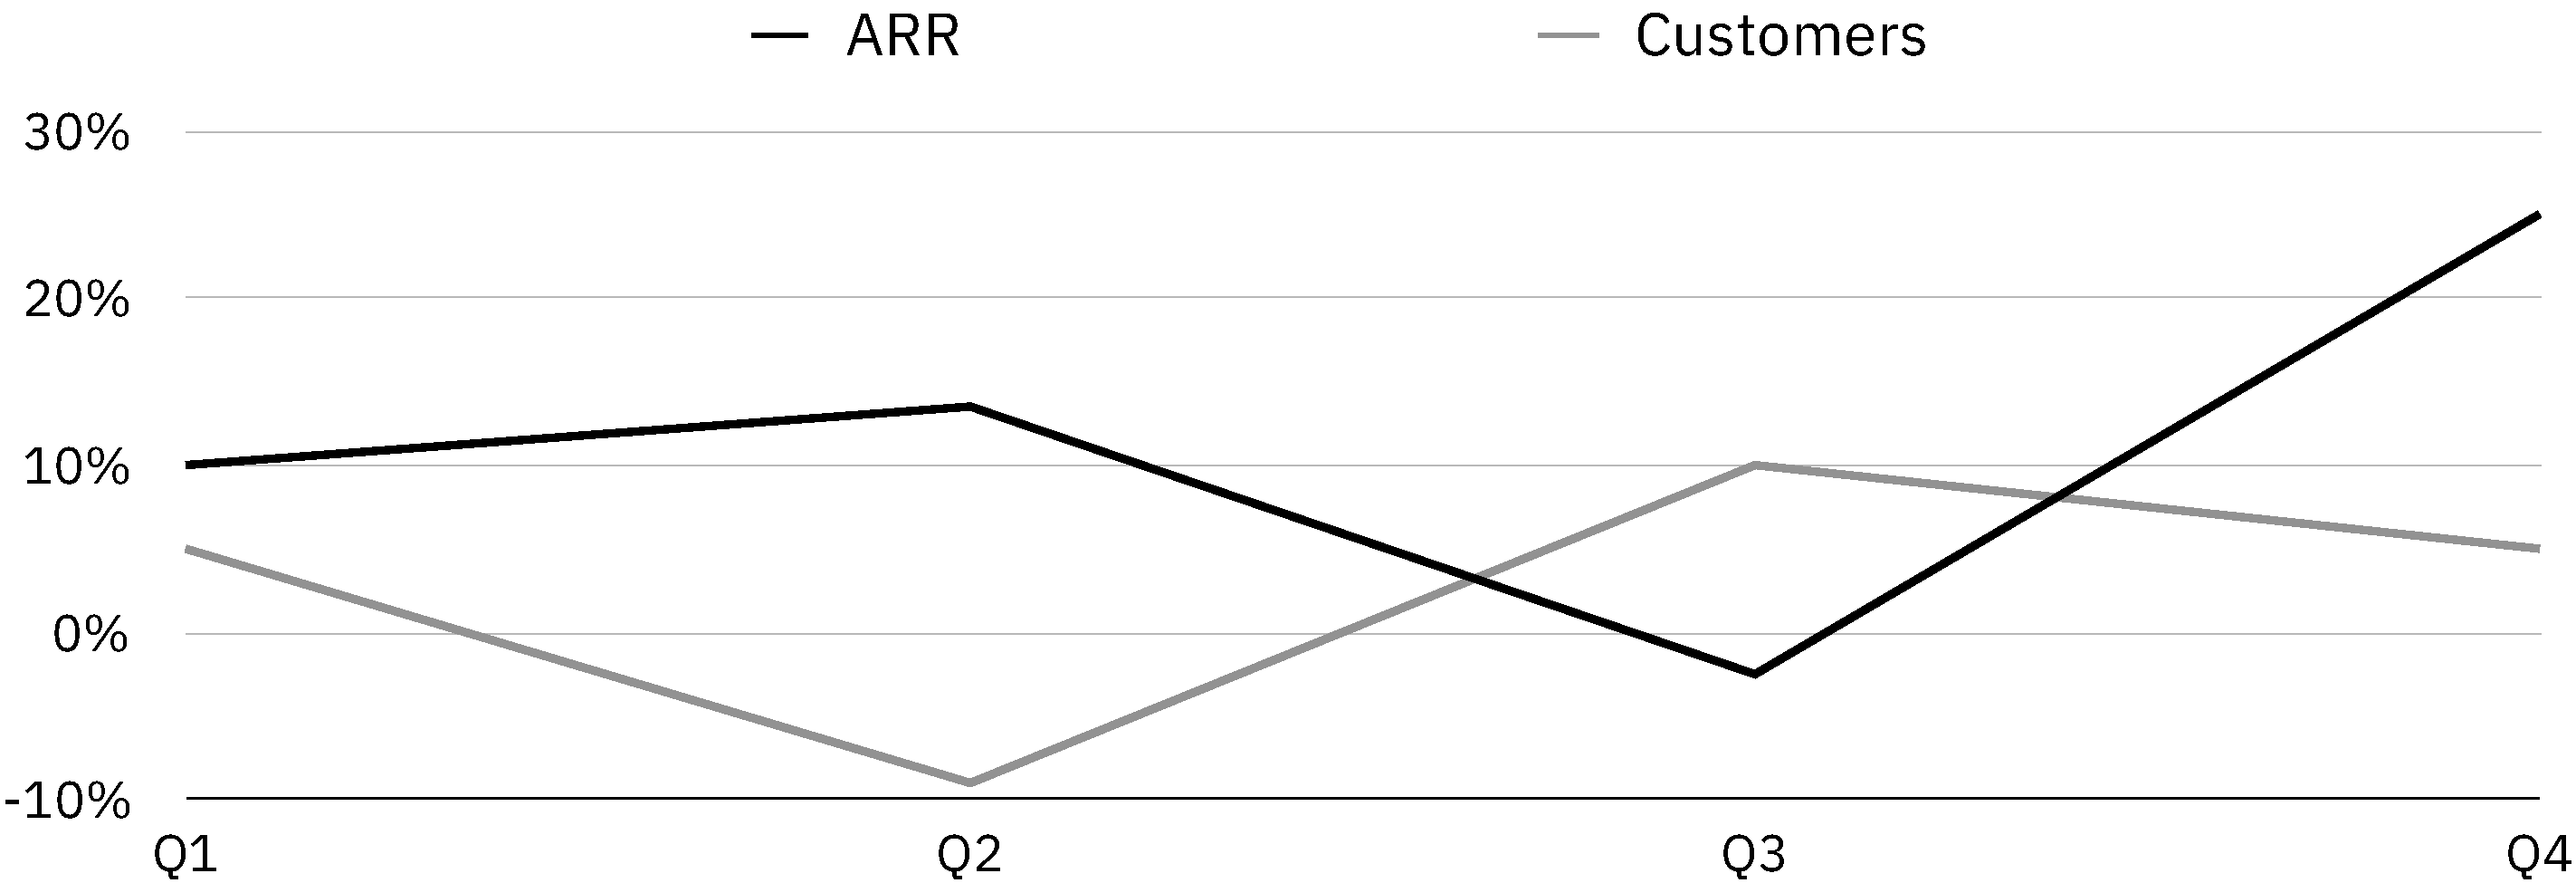
\includegraphics[width=\linewidth]{./include/ARR.pdf}
	\caption{Text block figure caption.}
	\label{fig:example} % Label for referencing this figure in the text automatically
\end{figure}

%------------------------------------------------

\begin{figure*} % Use the figure* environment for full width figures
	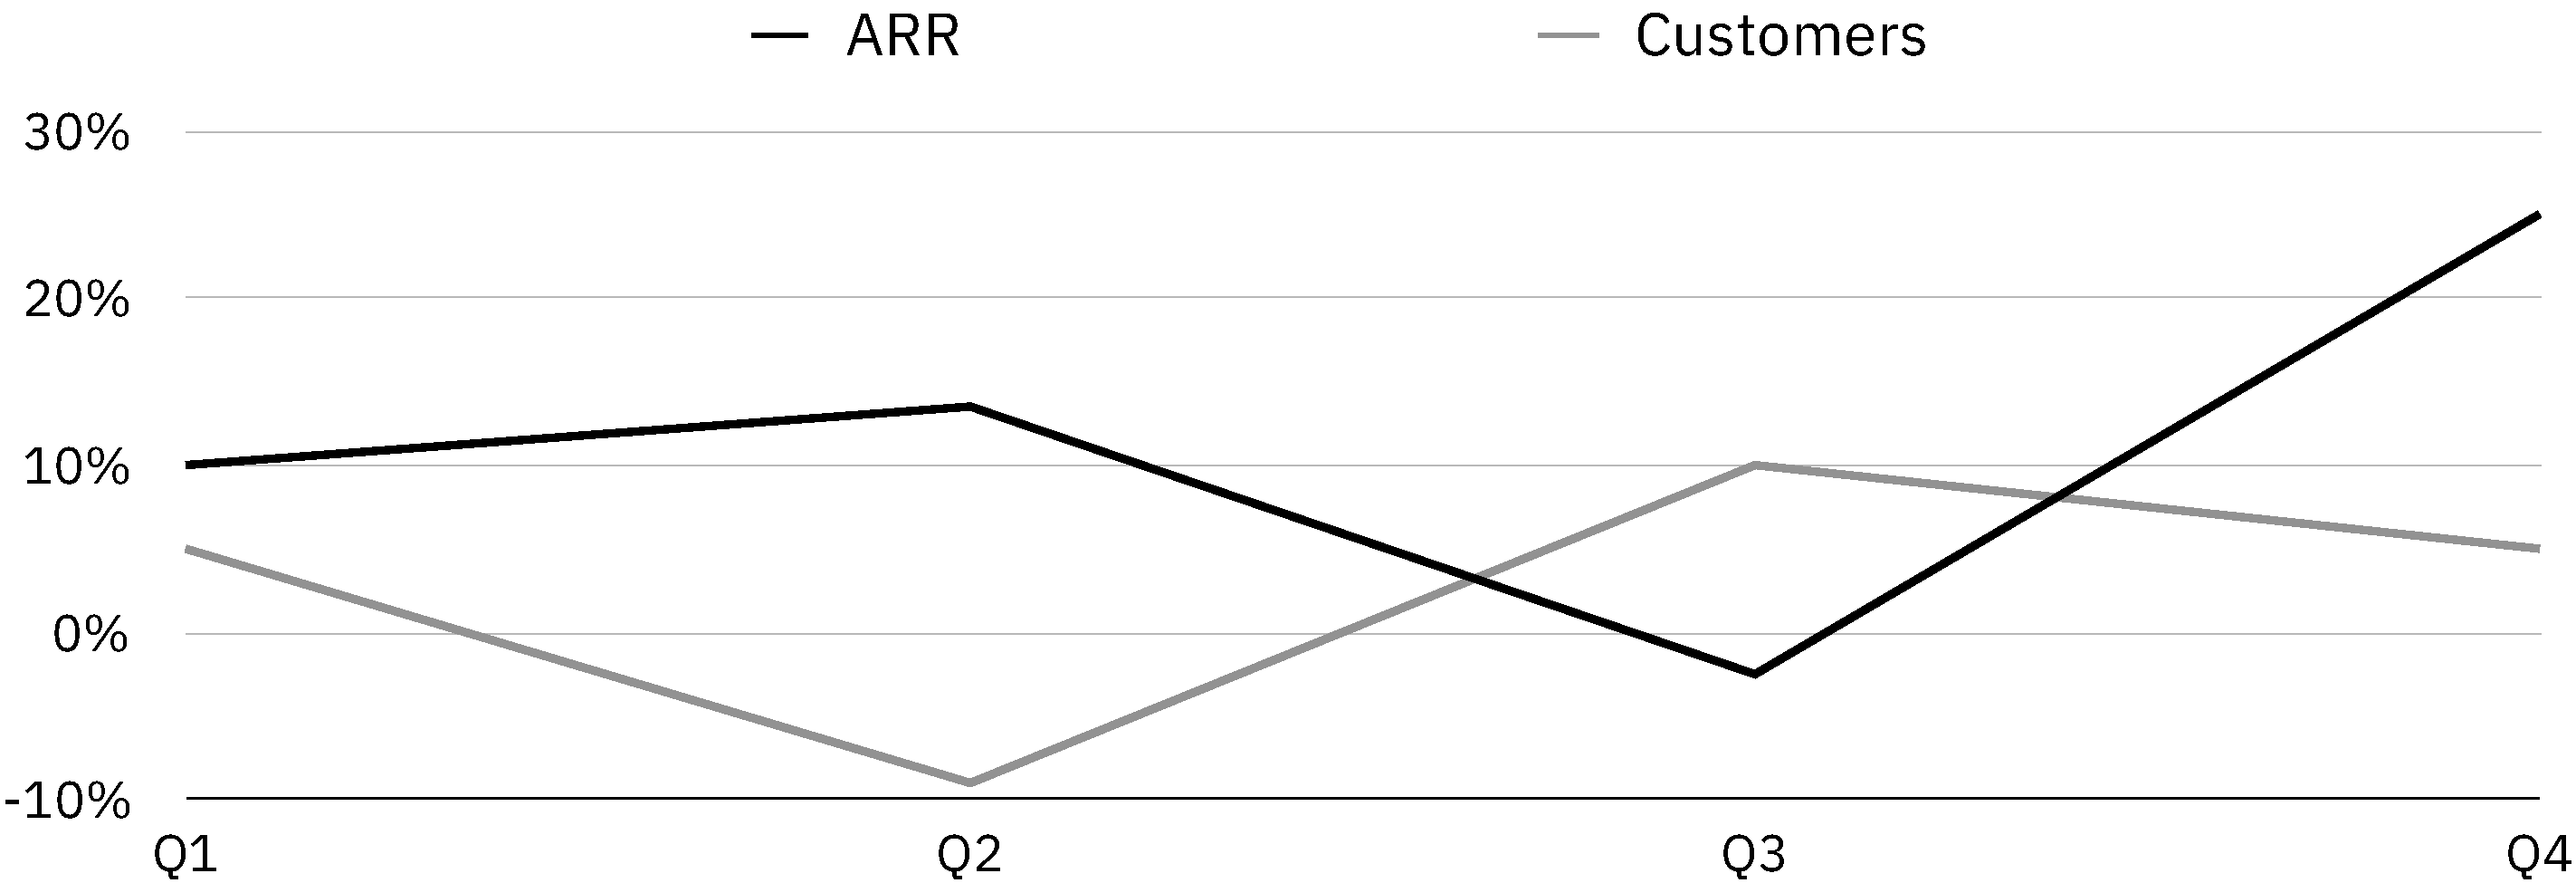
\includegraphics[width=\linewidth]{./include/ARR.pdf}
	\caption{Full width figure caption.}
\end{figure*}

%----------------------------------------------------------------------------------------
%	LISTS
%----------------------------------------------------------------------------------------

\section{List Examples}

\subsection{Bullet Point List}

\nonumsidenote{Bullet point lists can also be created in the margin. For these, we can remove the usual left margin to increase the available horizontal space:\\\medskip \begin{itemize}[leftmargin=*]\item Bullet item one. \item Bullet item two. \item Bullet item three.\end{itemize}}Lorem ipsum dolor sit amet, consectetur adipiscing elit. Praesent porttitor arcu luctus, imperdiet urna iaculis, mattis eros. Pellentesque iaculis odio vel nisl ullamcorper, nec faucibus ipsum molestie. Sed dictum nisl non aliquet porttitor.

\begin{itemize}
	\item First bullet point item
	\begin{itemize}
		\item First indented bullet point item
		\item Second indented bullet point item
		\begin{itemize}
			\item First second-level indented bullet point item
			\item Second second-level indented bullet point item
		\end{itemize}
		\item Third indented bullet point item
	\end{itemize}
	\item Second bullet point item
	\item Third bullet point item
\end{itemize}

Etiam vulputate arcu dignissim, finibus sem et, viverra nisl. Aenean luctus congue massa, ut laoreet metus ornare in. Nunc fermentum nisi imperdiet lectus tincidunt vestibulum at ac elit. Nulla mattis nisl eu malesuada suscipit.

%------------------------------------------------

\subsection{Numbered List}

\nonumsidenote[-2.5cm]{Numbered lists can also be created in the margin. For these, we can remove the usual left margin to increase the available horizontal space:\\\medskip \begin{enumerate}[leftmargin=*]\item Numbered item one. \item Numbered item two. \item Numbered item three.\end{enumerate}}Lorem ipsum dolor sit amet, consectetur adipiscing elit. Praesent porttitor arcu luctus, imperdiet urna iaculis, mattis eros. Pellentesque iaculis odio vel nisl ullamcorper, nec faucibus ipsum molestie. Sed dictum nisl non aliquet porttitor.

\begin{enumerate}
	\item First numbered item
	\begin{enumerate}
		\item First indented numbered item
		\item Second indented numbered item
		\begin{enumerate}
			\item First second-level indented numbered item
			\item Second second-level indented numbered item
		\end{enumerate}
		\item Third indented numbered item
	\end{enumerate}
	\item Second numbered item
	\item Third numbered item
\end{enumerate}

Etiam vulputate arcu dignissim, finibus sem et, viverra nisl. Aenean luctus congue massa, ut laoreet metus ornare in. Nunc fermentum nisi imperdiet lectus tincidunt vestibulum at ac elit. Nulla mattis nisl eu malesuada suscipit.

%------------------------------------------------

\subsection{Description List}

\nonumsidenote{Description lists can also be created in the margin:\\\medskip \begin{description}\item[A1] Description item one. \item[B1] Description item two. \item[C1] Description item three.\end{description}}Lorem ipsum dolor sit amet, consectetur adipiscing elit. Praesent porttitor arcu luctus, imperdiet urna iaculis, mattis eros. Pellentesque iaculis odio vel nisl ullamcorper, nec faucibus ipsum molestie. Sed dictum nisl non aliquet porttitor.

\begin{description}
	\item[Item One] Lorem ipsum dolor sit amet, consectetur adipiscing elit. Praesent porttitor arcu luctus, imperdiet urna iaculis, mattis eros. Pellentesque iaculis odio vel nisl ullamcorper, nec faucibus ipsum molestie.
	\item[Item Two] Sed dictum nisl non aliquet porttitor.
	\begin{description}
		\item[Subitem] Maecenas consectetur metus at tellus finibus condimentum. Proin arcu lectus, ultrices non tincidunt et, tincidunt ut quam. Integer luctus posuere est, non maximus ante dignissim quis.
		\begin{description}
			\item[Subsubitem] Maecenas consectetur metus at tellus finibus condimentum. Proin arcu lectus, ultrices non tincidunt et, tincidunt ut quam. Integer luctus posuere est, non maximus ante dignissim quis.
	\end{description}
	\end{description}
	\item[Item Three] Etiam vulputate arcu dignissim, finibus sem et, viverra nisl. Aenean luctus congue massa, ut laoreet metus ornare in. Nunc fermentum nisi imperdiet lectus tincidunt vestibulum at ac elit. Nulla mattis nisl eu malesuada suscipit.
\end{description}

Etiam vulputate arcu dignissim, finibus sem et, viverra nisl. Aenean luctus congue massa, ut laoreet metus ornare in.

%----------------------------------------------------------------------------------------
%	REFERENCING CITATIONS
%----------------------------------------------------------------------------------------

\section{Referencing Citations}

This statement requires citation \autocite{Smith:2024jd}.

This statement requires multiple citations \autocite{Smith:2024jd, Smith:2023qr}.

This short citation is in the margin\sidecite{Smith:2023qr}.

This long citation is in the margin\fullsidecite{Smith:2024jd}.

This statement has an in-text citation: \textcite{Smith:2024jd}.

%----------------------------------------------------------------------------------------
%	LINKS
%----------------------------------------------------------------------------------------

\section{Link Examples}

This is a URL link: \href{https://www.duckduckgo.com}{DuckDuckGo}.\nonumsidenote{Links can be clicked in the PDF to navigate to the linked website or email address.}

This is a email link: \href{mailto:example@example.com}{example@example.com}.

This is a monospaced URL link: \url{https://duckduckgo.com}.


%----------------------------------------------------------------------------------------
%	CODE
%----------------------------------------------------------------------------------------

\section{Displaying Code}

The block below is a code listing. It displays code in an easy to use way with line numbers for quick reference to specific parts of the code.

\begin{lstlisting}
{
	"city": [
		{
			"id": 1,
			"name": "Toronto",
			"country": "Canada",
			"population": 6200000
		},
		{
			"id": 2,
			"name": "New York",
			"country": "United States of America",
			"population": 8800000
		}
	]
}
\end{lstlisting}

%----------------------------------------------------------------------------------------
%	 REFERENCES/BIBLIOGRAPHY
%----------------------------------------------------------------------------------------

\newpage

\addcontentsline{toc}{section}{Reference List} % Add the bibliography to the table of contents

\begin{twothirdswidth} % Content in this environment to be at two-thirds of the whole page width
	\printbibliography[title=Reference List] % Output the bibliography with a custom section title
\end{twothirdswidth}

%----------------------------------------------------------------------------------------
%	APPENDICES
%----------------------------------------------------------------------------------------

\newpage

\section*{Appendices}

\begin{appendices}

\section{Appendix Section}

Lorem ipsum dolor sit amet, consectetur adipiscing elit. Aliquam auctor mi risus, quis tempor libero hendrerit at. Duis hendrerit placerat quam et semper. Nam ultricies metus vehicula arcu viverra, vel ullamcorper justo elementum. Pellentesque vel mi ac lectus cursus posuere et nec ex. Fusce quis mauris egestas lacus commodo venenatis. Ut at arcu lectus. Donec et urna nunc. Morbi eu nisl cursus sapien eleifend tincidunt quis quis est. Donec ut orci ex. Praesent ligula enim, ullamcorper non lorem a, ultrices volutpat dolor. Nullam at imperdiet urna. Pellentesque nec velit eget euismod pretium.

\section{Appendix Section}

Lorem ipsum dolor sit amet, consectetur adipiscing elit. Aliquam auctor mi risus, quis tempor libero hendrerit at. Duis hendrerit placerat quam et semper. Nam ultricies metus vehicula arcu viverra, vel ullamcorper justo elementum. Pellentesque vel mi ac lectus cursus posuere et nec ex. Fusce quis mauris egestas lacus commodo venenatis. Ut at arcu lectus. Donec et urna nunc. Morbi eu nisl cursus sapien eleifend tincidunt quis quis est. Donec ut orci ex. Praesent ligula enim, ullamcorper non lorem a, ultrices volutpat dolor. Nullam at imperdiet urna. Pellentesque nec velit eget euismod pretium.

\section{Appendix Section}

Lorem ipsum dolor sit amet, consectetur adipiscing elit. Aliquam auctor mi risus, quis tempor libero hendrerit at. Duis hendrerit placerat quam et semper. Nam ultricies metus vehicula arcu viverra, vel ullamcorper justo elementum. Pellentesque vel mi ac lectus cursus posuere et nec ex. Fusce quis mauris egestas lacus commodo venenatis. Ut at arcu lectus. Donec et urna nunc. Morbi eu nisl cursus sapien eleifend tincidunt quis quis est. Donec ut orci ex. Praesent ligula enim, ullamcorper non lorem a, ultrices volutpat dolor. Nullam at imperdiet urna. Pellentesque nec velit eget euismod pretium.

\end{appendices}

%----------------------------------------------------------------------------------------

\end{document}
